\chapter{Evaluation}

\section{Customer Requirements}


\subsection{Objective Evaluation}

Below is a list of all my general and specific objectives that I set myself in the analysis section. In this section I will determine whether I have met all of these objectives and the reasoning behind it. The subsections with *NEW* in the title are objectives that I did not identify in my analysis section; however during the course of my implementation, I attempted to meet the objectives. 

\subsubsection{Aesthetically pleasing, easy to navigate GUI.} %Need feedback

This objective has been met.

From the bar chart in Figure \ref{fig:AestheticsGraph} on page \pageref{fig:AestheticsGraph}, which gives a bar chart analysis of all of the questionnaire responses to asking about the aesthetics and ease of navigating the program. you can see that 60\% of the questionnaires that were filled in responded that they strongly agree that the program is aesthetically pleasing and easy to navigate, with a further 40\% agreeing. Making a total of 100\% positive feedback in response to the question posed. Therefore I believe that my program is aesthetically pleasing and easy to navigate.




\subsubsection{Videos organised and filtering capabilities.}

This objective has been partially met. 

The video links (tricks tutorial link) are organised in the tricks table in the order of TrickID; however there are no fitering capabilities implemented in the program at this stage. 


\begin{figure}[H]
    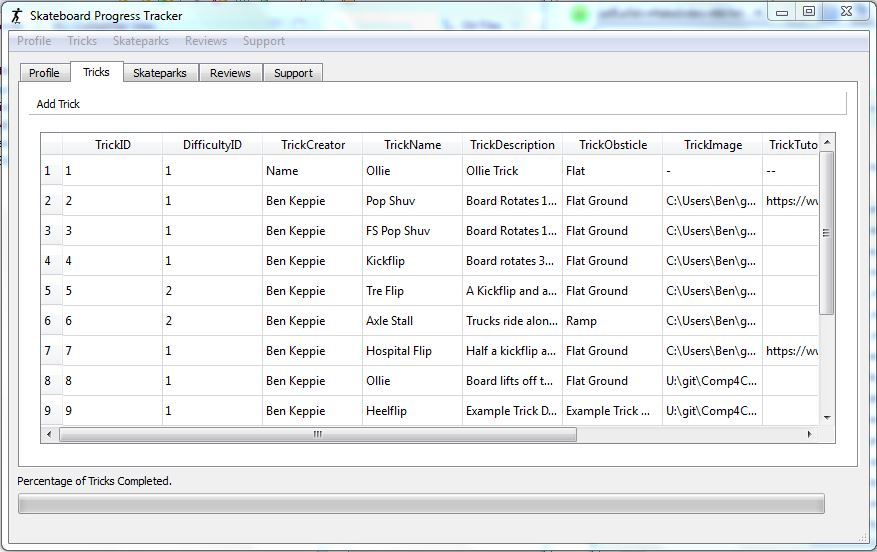
\includegraphics[width=\textwidth]{./Evaluation/images/OrganisedTricks.jpg}
    \caption{Tricks Organised by TrickID} \label{fig:TricksOrganised}
\end{figure}

The figue above shows that the video links have been organised by TrickID. With the first TrickID being at the top of the table and the last being at the bottom; however, from the figure above you can see that there are no filtering capabilities within the Tricks tab which contribute to the functionality of filtering the tricks table.




\subsubsection{Correct and accurate mapping to the skate parks/spots.}

This objective has been met.

I am using the most recent Google maps image available and therefore the roads in between skate parks and spots are up to date.



\subsubsection {Correct directions from current location to skate park/ spot on the map.}

This objective has not been met.

Currently my program has no functionality which allows the user to plot a route which gives step by step instructions.



\subsubsection{Non-biased reviews.}

This objective has been met to an extent. 

As the program is currently a single user application, the only reviews that will be in place will be the reviews that my client adds. Therefore the only way the review would be biased is if my client specifically made a biased review. 



\subsubsection{Clear database with a list of tricks in.} %Need feedback

This objective has been met.

My bar chart in Figure \ref{fig:TricksTableGraph} on page \pageref{fig:TricksTableGraph} shows that 80\% of the feedback that I received on my questionnaire agreed with the fact that it was easy to read, with a further 20\% of feedback strongly agreeing which leaves a 100\% turn over of positive feedback.


\begin{figure}[H]
    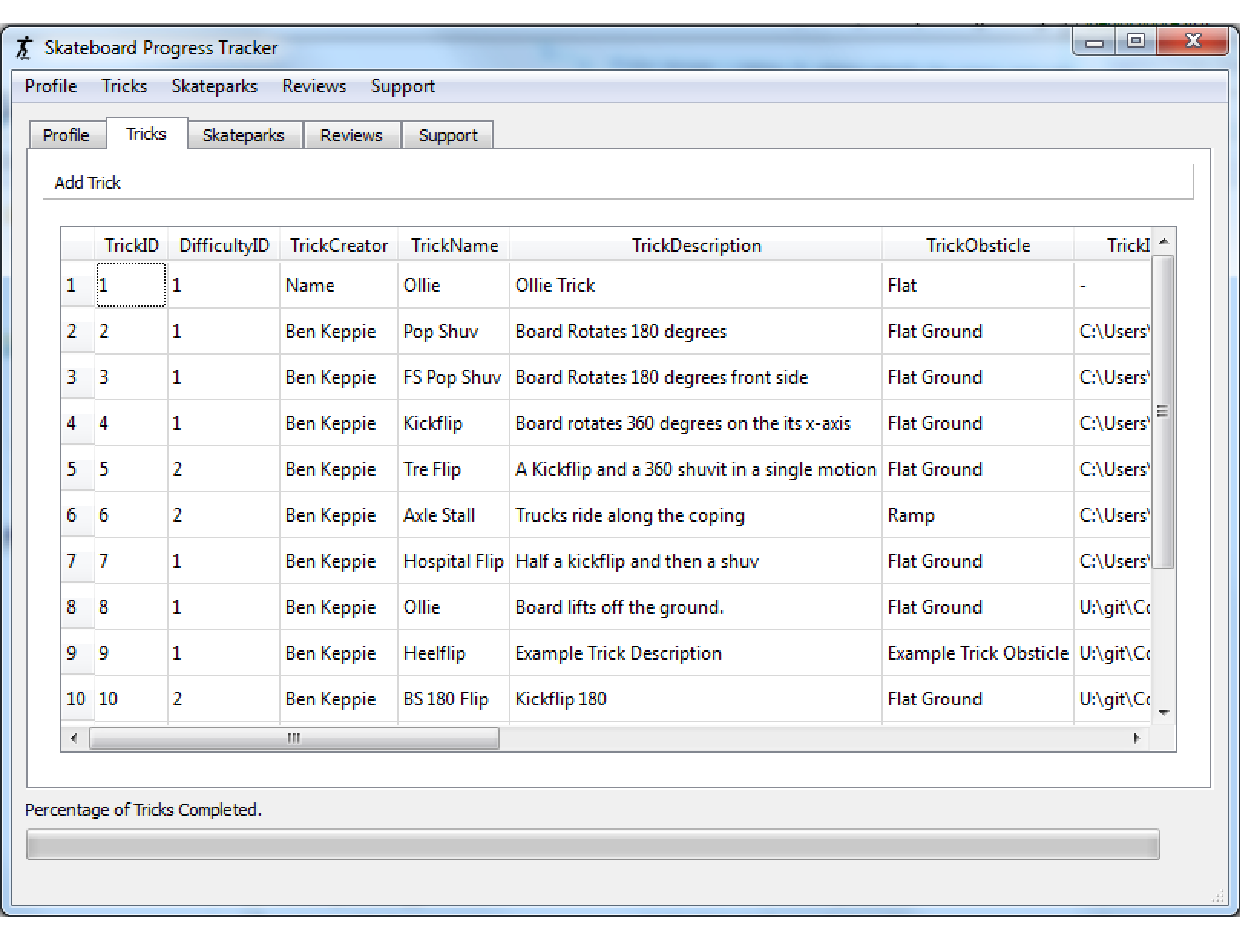
\includegraphics[width=\textwidth]{./Evaluation/images/TricksTableNFS.pdf}
    \caption{Tricks Table with a List of Tricks in} \label{fig:TricksTableEX}
\end{figure}

The figure above shows my table with my list of tricks in.







\subsubsection{ Easy to filter through tricks known.}

This objective has not been met. 

As discussed before, filtering capabilities have not been implemented in this version of the program.



\subsubsection {Display status bar messages at appropriate times to inform the user of changes *NEW*} %FEEDBACK

This objective has been met.

I have decided this as 100\% of my questionnaires that I received back strongly agree with the statement. This is shown by my questionnaire section (\ref{QSub}) of my evaluation on page \pageref{QSub}.



\subsubsection {Allow for the user to contact the developer *NEW*}

This objective has been met.


\begin{figure}[H]
    \includegraphics[width=\textwidth]{./Evaluation/images/Contactsupport.jpg}
    \caption{Contacting Developer Form} \label{fig:ContactSupportEVD}
\end{figure}

The figure above shows the form in the support tab which users can fill in, in order to contact the developer with any problems or queries about the program.



\subsubsection {Ensure that the profile picture can be changed easily *NEW*} 

This objective has been met.

This is backed up by the feedback received from my questionnaire were everyone who responded, replied with 'yes' to the question asking if the profile picture was easy to change. My questionnaire responses can be found in section \ref{QSub} on page \pageref{QSub}.



\subsubsection {Ensure that the profile name can be edited easily *NEW*} %Need feedback

This objective has been met.

This is backed up by the feedback received from my questionnaire were everyone who responded, replied with 'yes' to the question asking if the profile picture was easy to change. My questionnaire responses can be found in section \ref{QSub} on page \pageref{QSub}.



\subsubsection {Ensure that the profile email can be edited easily *NEW*} %Need feedback

This objective has been met.

This is backed up by the feedback received from my questionnaire were everyone who responded, replied with 'yes' to the question asking if the profile picture was easy to change. My questionnaire responses can be found in section \ref{QSub} on page \pageref{QSub}.




\subsubsection {Ensure that videos can be filtered by categories. e.g easy, medium, hard tricks.}

This objective hasn't been met.

As discussed before, filtering capabilities have not been implemented in this version of the program.




\subsubsection {Ensure that videos load correctly and are linked to the right video.}

This objective has been met.

 I have used a regular expression to validate an official YouTube video link, and on top of that referential integrity has been enforced in the database so that the tutorial link will be assigned to the trick that it was added to by the user. 




\subsubsection {Ensure that videos are displayed at the correct size/resolution that the monitor of the computer is.}

This objective has been met.

As the videos are viewed in the computers default web browser, the videos will be shown in the correct size/resolution that the monitor is.



\subsubsection {Ensure the database can add, edit and remove trick data (Name, description, image, completed status and tutorial link).}

This objective has been met.

The program is able to graphically add and delete trick data and within the command line interface, the trick data can be edited. This is proven by the testing section of my coursework (Table \ref{tab:TestingResults} on page \pageref{tab:TestingResults})

\subsubsection {Ensure that the database is displayed correctly inside the application at all resolutions.}

This objective has been met.

I have used a QTableView object within my graphical user interface which has allowed the database to stay in the layout. The program is also displayed at the resolution of the monitor that is is run on and therefore is displayed at the appropriate resolution.

\subsubsection {Ensure that the tricks are marked by how hard they are by a three way scale of: Easy, Medium or Hard.}

This objective has been met.

\begin{figure}[H]
    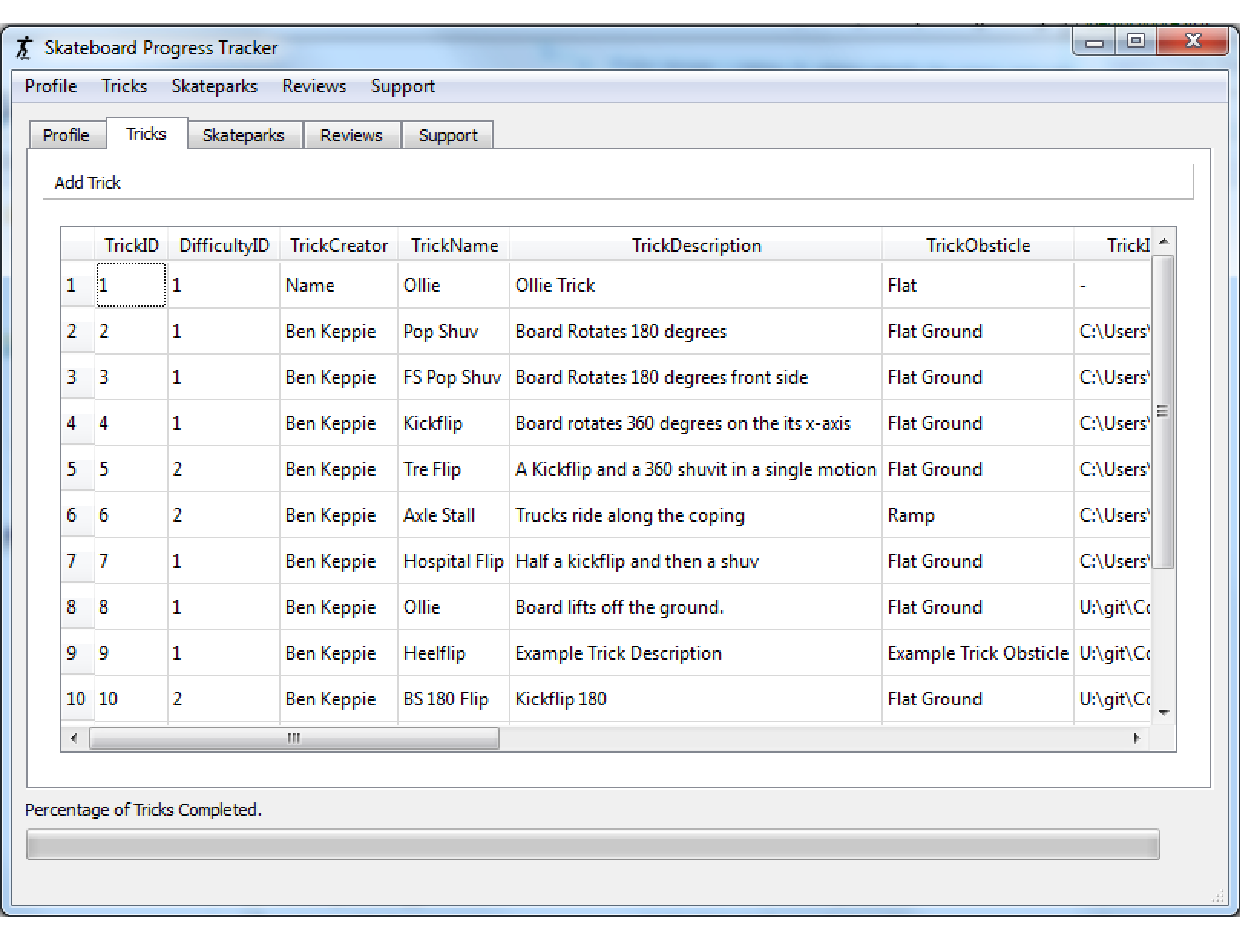
\includegraphics[width=\textwidth]{./Evaluation/images/TricksTableNFS.pdf}
    \caption{Tricks Marked With a Difficulty} \label{fig:TricksTableDiff}
\end{figure}

In the figure above, the table shows that each individual trick has a trick difficulty. The trick difficulty is a number which corresponds to the three way scale.

\begin{itemize}
\item $1 = Easy$
\item $2 = Medium$
\item $3 = Hard$
\end{itemize}


\subsubsection {Ensure a checkbox is by the side of a trick to represent whether the user has completed that trick or not.}

This objective hasn't been met.

I did not get time to implement the check box functionality into the QTableView.

\subsubsection {Ensure there is a search bar for a specific trick name.}

This objective hasn't been met.

I did not get time to implement the searching for a tricks functionality in the tricks tab.

\subsubsection {Ensure there are filters for tricks e.g Switch trick filters.}

This objective hasn't been met.

As discussed before, filtering capabilities have not been implemented in this version of the program.




\subsubsection {Ensure that the map is accurate to current roads.}

This objective has been met.

I am using the most recent Google maps image available and therefore the maps object is as up to date with current roads as possible. The way that I have implemented my Google maps object means that the map will be automatically updated to the most recent version of Google maps.

\subsubsection {Ensure location of the user is not revealed to anyone else.}

This objective has been met.

The program doesn't take in the users current location and therefore it isn't stored and cannot be found.

\subsubsection {Ensure that the current location marker is accurate.}

This objective hasn't been met.

My program hasn't got a current location marker implemented as the computers used to program my system did not have access to any location functionality.

\subsubsection {Ensure that when giving directions to skate parks from your current location that the mapping route is correct and on viable roads. }

This objective hasn't been met.

I did not get time to add location to location directions whilst implementing my program.

\subsubsection {Ensure that the program can mark skate park locations.}

This objective has been met.

The user can mark skatepark locations by left clicking on the mouse whilst the cursor is inside the Google maps object. The coordinates will only be recorded for adding purposes when the map is in editing mode.

\begin{figure}[H]
    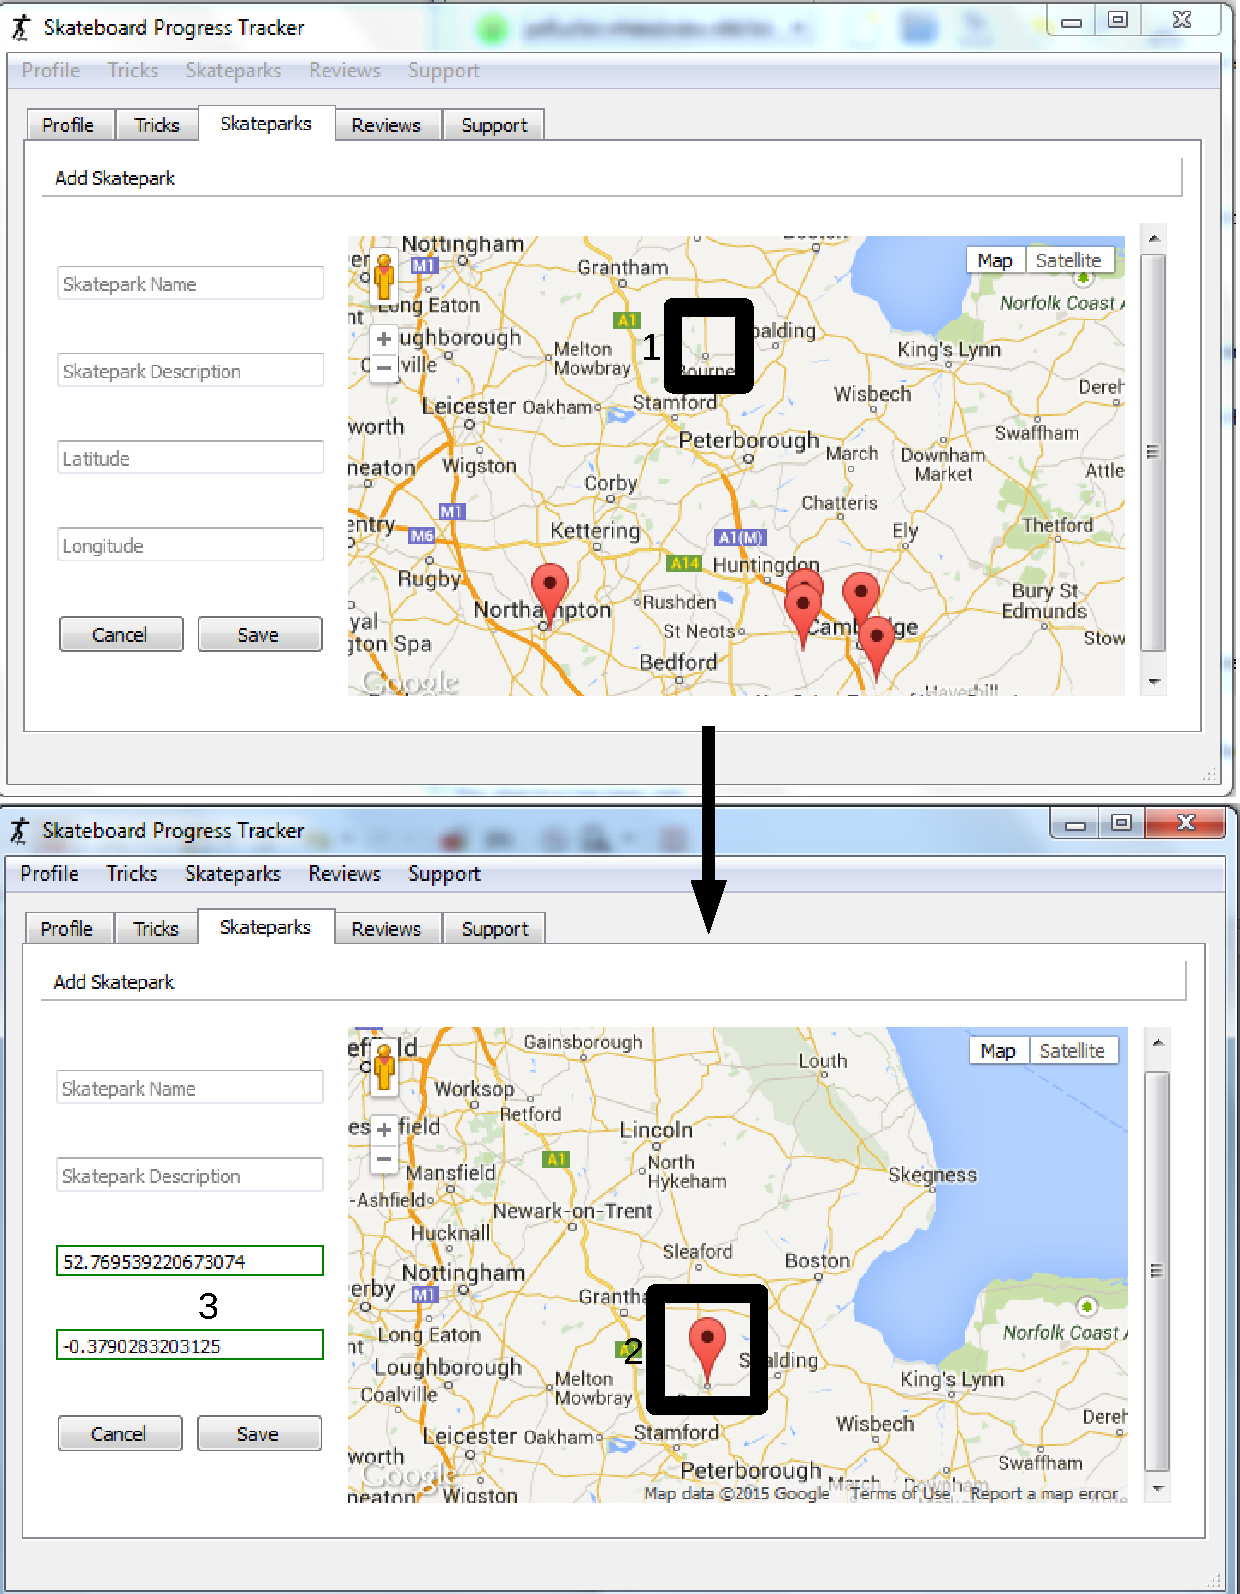
\includegraphics[width=\textwidth]{./Evaluation/images/MarkerEvidence.pdf}
    \caption{Marking a Skatepark Location} \label{fig:MarkerEvidence}
\end{figure}

The figure above shows the process of left clicking on a specific location and a marker appearing. The numbers annotated on the image above correspond to an explanation below.

\begin{enumerate}
\item Left click on a specific location.
\item A Google maps marker appears at that location.
\item If in edit mode, the longitude and latitude of that skatepark will appear in the coordinate fields.
\end{enumerate}

This objective is also backed up by the 100\% feedback saying that it is easy to add a skatepark. My questionnaire responses can be found in section \ref{QSub} on page \pageref{QSub}.




\subsubsection {Ensure no biased reviews are posted to the app and that they're moderated before they are universally posted.}

This objective has been met to an extent.

As the program is currently a single user application, the only reviews that will be in place will be the reviews that my client adds. Therefore the only way the review would be biased is if my client specifically made a biased review. 



\subsubsection {Ensure the program runs fast without lag when navigating between areas of the application.}  %Need Feedback.

This objective has been met.

For my questionnaire users were given a choice to select a number from 1 - 10 corresponding to the response of the program to activities ($1 = Slow$ and $10 = Fast$) all of the questionnaires that I received back gave the highest possible mark of 10. This leads me to believe that my program doesn't have any lag and runs fast. Whilst using my program I have also experienced the same speeds in response to activities.








\section{Effectiveness}

\subsection{Fully Effective Solutions}



	\subsubsection{Correct and accurate mapping to the skateparks/ spots.}

As the Google maps object is automatically updated whenever Google updates the map, this objective is very effective. This automatic update is able to occur as I have embedded a Google maps object which is taken from the most recent version of Google maps. 

	\subsubsection{Display status bar messages at appropriate times to inform the user of changes *NEW*}

100\% of my questionnaires that I received back strongly agree with the statement. This is shown by my questionnaire section (\ref{QSub}) of my evaluation on page \pageref{QSub}. This suggests that my solution is fully effective for this objective. 

	\subsubsection{Allow for the user to contact the developer *NEW*}

My solution for this objective was to have a form on a support tab. I decided to implement this objective in this format as this is standard in the computing industry. This solution was approved by my client and questionnaire participants, as supported by the 100\% agreement with the statement that it's easy to contact support. Therefore this objective is fully effective.

	\subsubsection{Ensure that the profile picture can be changed easily *NEW*}

Changing the profile picture involves pressing 'Change Picture' on the status bar of the profile tab and then selecting an image file from the file dialog that appears. The profile picture then automatically changes to the newly chosen image. This was a good solution to the objecting as websites which people commonly use, such as Facebook, uses this method for changing the profile picture. This may explain the fact that everybody that carried out the questionnaire agreed that the profile picture was easy to change. Therefore I feel this solution is very effective.

	\subsubsection{Ensure that the profile name can be edited easily *NEW*}

Changing the profile name involves entering edit mode and changing the name fields. This was said to be an easy way to change the name, as shown by my feedback in section (\ref{QSub}) on page \pageref{QSub}. Therefore I feel this solution is effective.

	\subsubsection{Ensure that the profile email can be edited easily *NEW*}

Changing the profile email involves entering edit mode and changing the email field. This was said to be an easy way to change the email, as shown by my feedback in section (\ref{QSub}) on page \pageref{QSub}. Therefore I feel this solution is effective.

	\subsubsection{Ensure that videos load correctly and are linked to the right video.}	

As long as the device running the program has internet access and a web browser which allows them to play YouTube videos, the video will load correctly. This isn't a solution I specifically programmed, but it is an effective way of adding tutorial videos to tricks. Referential integrity ensures that videos stay linked to the correct trick.



	\subsubsection{Ensure that the database is displayed correctly inside the application at all resolutions.}

As I have a series of layouts which hold my tables which display data from my database, the user is unable to modify and change the table so that it is incorrectly displayed inside the application. Therefore the way that I have programmed this is extremely effective.

	\subsubsection{Ensure that the map is accurate to current roads.}

As the Google maps object is automatically updated whenever Google updates the map, this objective is very effective. This automatic update is able to occur as I have embedded a Google maps object which is taken from the most recent version of Google maps. 

	\subsubsection{Ensure location of the user is not revealed to anyone else.}

As location data is never taken in by the program, it would be impossible for anyone to find out the location of the user. Therefore the objective is as effective as it can possibly be at this moment in time; however when features involving location are introduced, the solution will have to change to protect location data within an encrypted database. 

	\subsubsection{Ensure that the program can mark skate park locations.}

I believe that this objective is extremely effective. All of the feedback received said that it was easy to mark skate park locations and therefore the way in which skate parks are added is effective. I chose to program the way to place a marker by inducing a left mouse click. I did this because this is the most intuitive and common way to interact with a computer. This therefore made a very effective solution to the objective.

	\subsubsection{Ensure the program runs fast without lag when navigating between areas of the application.}

As discussed before, all of my received feedback rated my application the fastest rating, therefore the way that I have implemented my program is extremely effective at efficiency of carrying out tasks.

\subsection{Not Fully Effective Solutions}

	\subsubsection{Aesthetically pleasing, easy to navigate GUI.}

My client has said that a bit more colour within the application would make the aesthetics of the program better, this can be found in Stuarts questionnaire, Figure \ref{fig:StuFeedback3} on page \pageref{fig:StuFeedback3}. Therefore my GUI is not currently fully effective.

\subsubsection{Clear database with a list of tricks in effectiveness}

Although my objective was met, two pieces of feedback suggested some improvements. This suggested that although the objective was met, the was that it was met could be carried out better. The first piece of feedback came from my client, Stuart. On question 4 on the questionnaire, he stated that it was clear when it was full screen or maximised. This piece of feedback is shown below.

\begin{figure}[H]
    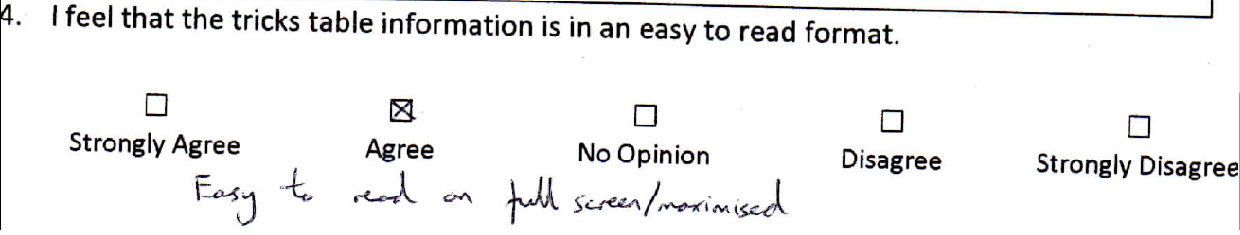
\includegraphics[width=\textwidth]{./Evaluation/images/StuTricks.pdf}
    \caption{Stu Tricks Table Feedback} \label{fig:StuTricksFeedback}
\end{figure}

 The two figures below show the table when not in full screen and when it's in full screen.

\begin{figure}[H]
    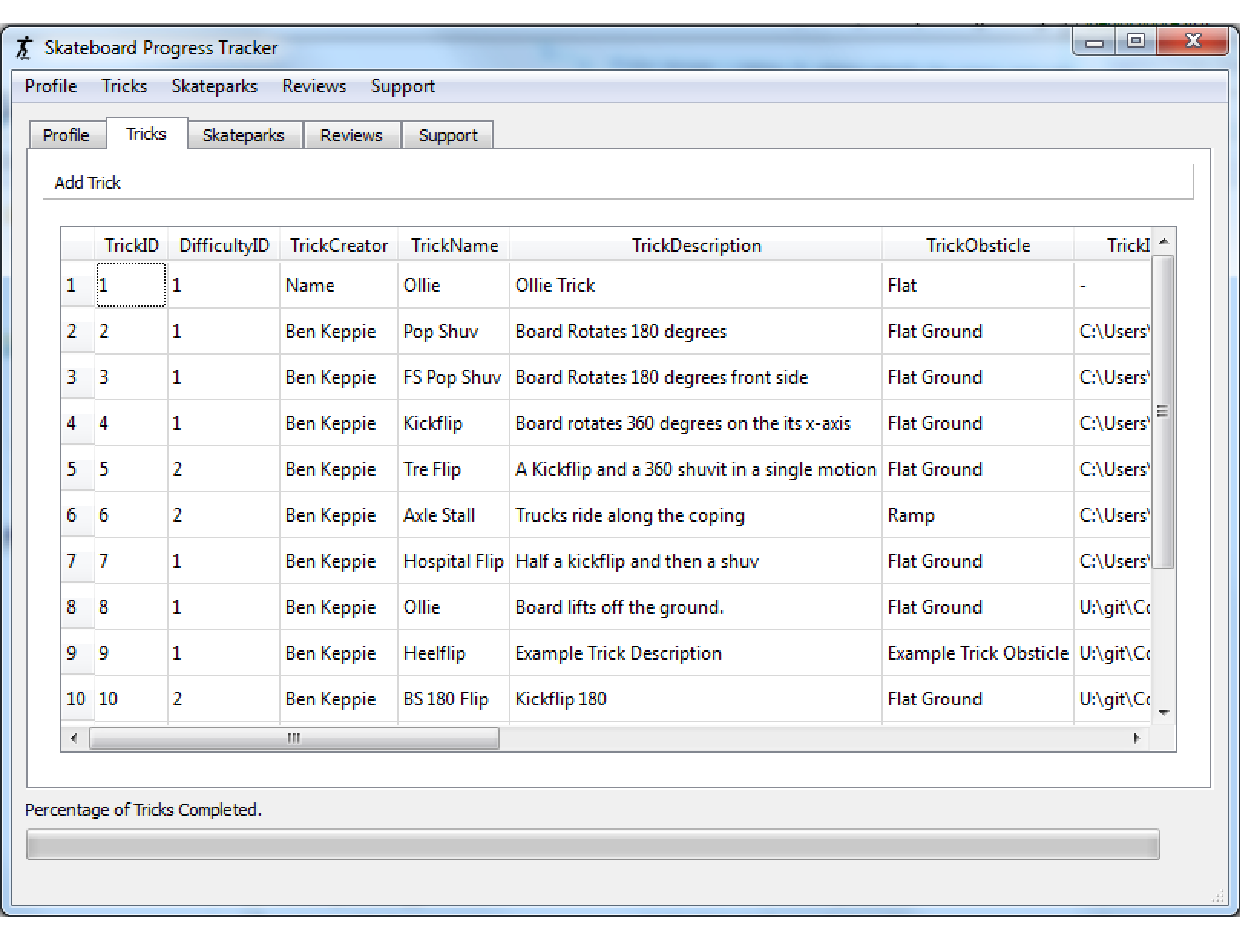
\includegraphics[width=\textwidth]{./Evaluation/images/TricksTableNFS.pdf}
    \caption{Tricks Table Not Full Screen} \label{fig:TricksTableNFS}
\end{figure}

\begin{figure}[H]
    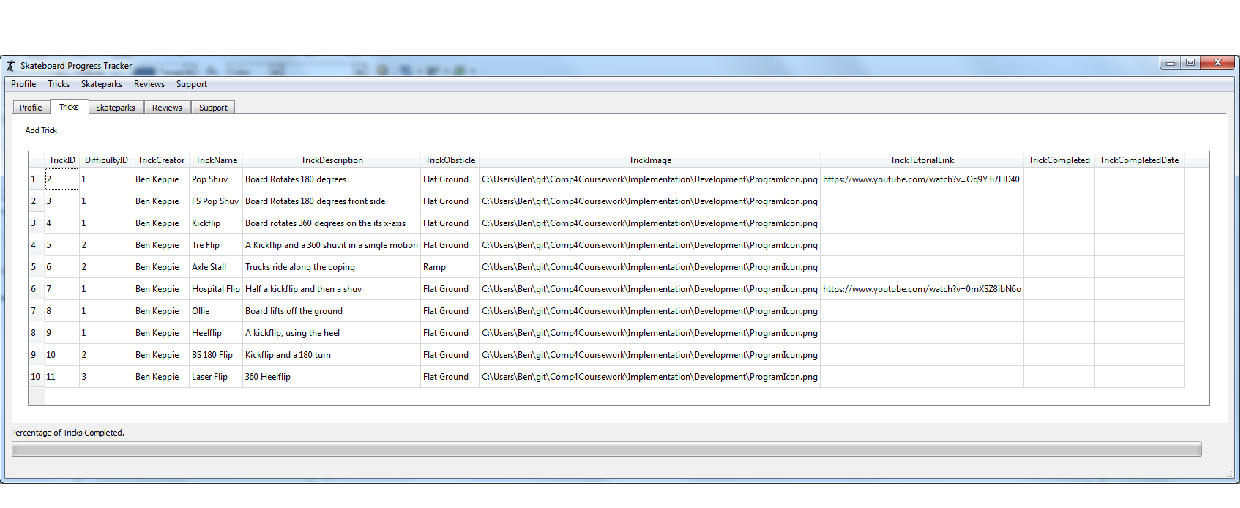
\includegraphics[width=\textwidth]{./Evaluation/images/TricksTableFS.pdf}
    \caption{Tricks Table Full Screen} \label{fig:TricksTableFS}
\end{figure} 

The other piece of feedback that I got was from Sues' feedback, where she said that it would be better to have the actual words for the difficulty of the trick rather than a corresponding number. This is shown below.

\begin{figure}[H]
    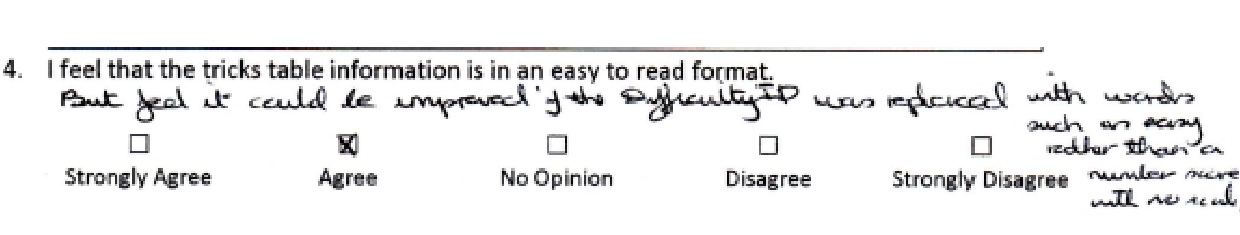
\includegraphics[width=\textwidth]{./Evaluation/images/SueTricks.pdf}
    \caption{Sue Tricks Table Feedback} \label{fig:SueTricksFeedback}
\end{figure}




\subsubsection{Non-biased Reviews}

As there is no way of filtering biased reviews from being added to the database, the current way of how reviews get added to the database are not completely biased proof. Although the system is a single user system, my client could still put a biased review into the database. However because of this single person system, this does not matter. In the future, however, this will matter and reviews will have to be monitored. Therefore in conclusion, currently the solution works, but by the time I implement a multi-user system the current way of adding reviews to the database will not be suitable.

\subsubsection{Ensure that the tricks are marked by how hard they are by a three way scale of: Easy, Medium or Hard.}

Although I have implemented a number system to correspond to the difficulty of a trick, my feedback form shown by Figure \ref{fig:SueFeedback1} on page \pageref{fig:SueFeedback1} states that it would be a lot easier for tricks to be marked by the words rather than a number rating system. This leads me to believe that my solution to that objective is not fully effective. I also agree that the program should display an English language trick difficulty scale so that the users of the program do not need to look up in the user manual what the data means.

	\subsubsection{Ensure the database can add, edit and remove trick data (Name,description, image, completed status and tutorial link).}

As editing trick information is only available in command line interface, the solution is not completely effective. In order for the solution to be fully effective I would have to implement an easy, intuitive way of editing trick information by interacting with the tricks table displayed in the tricks tab.

	\subsubsection{Ensure that videos are displayed at the correct size/resolution that the monitor of the computer is.}

As the videos are viewed in the computers default web browser, the videos will be shown in the correct size/resolution that the monitor is. I feel that this is a reasonable solution. However implementing a built in video player would probably be a more effective solution as all of the functionality will be integrated into the program. 











\section{Learnability}

My program doesn't need any prior knowledge in order to operate it. This means that I had to implement the program in a way which makes the program self explanatory. One example of this is that in my questionnaire I asked if the participant understood that the skatepark map was implemented so that the user can find new skateparks and spots. The feedback that I received shows that 100\% of the participants understood. This feedback was received from skaters and non-skaters alike. This shows that my program is easy to use.



\section{Usability}

	\subsection{Readability}

My programs text is presented on a white background with black text, this high contrast of colours allows for text within my program to be easily read. Backgrounds of similar shades have been specifically avoided in order to make the users experience of the program better due to an increased ease of readability. This is backed up by my 100\% positive feedback on the aesthetics of my program (Figure \ref{fig:AestheticsGraph} on page \pageref{fig:AestheticsGraph}).

I have not changed the size of the text in my program, and am therefore using the standard font size that comes with the PyQt module. This has been optimised for neat looking and an easy to read size for all monitor resolutions. 

The skateboard progress tracker contains the format of all text being formatted into layouts which has created a nicely formatted text platform. 

	\subsection{Navigability}

My program contains a tab format which allows for different information to be displayed in each tab. I named the tabs appropriately so that the user would easily be able to identify which tab they needed to be in, in order to carry out a particular function. For example, if you want to add a trick, you would click on the tricks tab as it is the most appropriate tab for carrying out that action.

I have used a familiar format for all programs. I have implemented a status bar with the functionality of a particular tab; however all functionality, from any tab, can be accessed by the menu bar. By selecting a function from a different tab from the menu bar, the user is taken to the tab with the functionality that they chose. This use of navigation shortcuts allows for ease of navigation.

	\subsection{Ease of Use}

I chose to implement the program in a way which makes the program self explanatory. In my questionnaire I asked if the participant understood that the skatepark map was implemented so that the user can find new skateparks and spots. The feedback that I received shows that 100\% of the participants understood. This shows that my program is easy to use.

\section{Maintainability}

	\subsection{Fixing Bugs}

As my code is self-documenting, due to the appropriate variable names and coding structure (as discussed in the system maintenance section of my coursework) my program will easily be able to have bugs fixed. The fact my code is split up over many different python files allows for ease of finding error locations and any complex code has a commented out section which explains what it does.

	\subsection{Changing Parameters}

As my code contains no global variables, changing the parameters shouldn't affect any other parts of the program unless that variable is used in a local state. 

	\subsection{Responding to New Requirements}

My program is split up into a modular structure, as each different class is a different python file the program will be easy to maintain whilst adding new requirements. 

	\subsection{Google Maps API}

Although Google maps code changes occasionally, I am led to believe that the code that I have used will not change. As the API key is my own personal key, the code will work as long as I leave my API key open.

\section{Suggestions for Improvement} 



	\subsection{Video Filtering Capabilities}

As I did not include video filtering capabilities in my first release of my program, I will add the ability to filter the tricks table in version 2.0 of the program. This will include a filtering choice of videos that are for easy, medium and hard tricks.


	\subsection{Current Location Data}

I was unable to originally implement the current location data; however if I continue to work on the program on a computer which enables location data I will add current location data. This will enable me to tailor the map to the user as well as map routes from the current location of the user.

	\subsection{Route Mapping Functionality in Google Maps}

Adding route mapping functionality into my program will allow the user to be able to easily map their journey to skateparks and spots. This functionality was initially wanted by my client, and has requested that I implement it in version 2.0 of my program.

	\subsection{Trick Filtering Capabilities}

As I did not include trick filtering capabilities in the first release, I am releasing it in in version 2.0. This will include filtering capabilities on all of the trick headings. For example, you will be able to filter through different tricks with a specific trick obstacle.

	\subsection{Checkboxes Inside Tricks Table}

Adding checkboxes into the trick table will not only allow the user to keep track of the tricks that they are able to perform, but it will also allow the progress bar at the bottom of the profile and tricks tab to function correctly. This was meant to be originally implemented in version 1.0 but unfortunately I was not able to due to the lack of time I had to complete my program.

	\subsection{Trick Searching Capabilities}

Searching for tricks in the trick table will be an added functionality, implemented in version 2.0 of my program.

	\subsection{Multi-User Platform}

Making a multi-user platform will allow for reviews made by other people to be displayed on everyones application. This will allow me to completely satisfy many of my initial objectives. For example, I will be able to moderate reviews posted by users.

	\subsection{Multi-Device Platform}

Stuart brought to my attention that it would be pretty useful if he could have the application on his phone so that he could use it on the go with ease. Creating an android application for the skateboarding progress tracker is an improvement that could be implemented.

	\subsection{Spelling Correction}

As illustrated by my clients feedback, on the tricks table and the 'add trick' form, I have spelled 'obstacle' as 'obsticle'. In version 2.0 of the skateboard progress tracker, this spelling mistake will be fixed.



\section{End User Evidence}

\subsection{Questionnaires} \label{QSub}

\subsubsection{Client Feedback Questionnaire} 


\begin{figure}[H]
    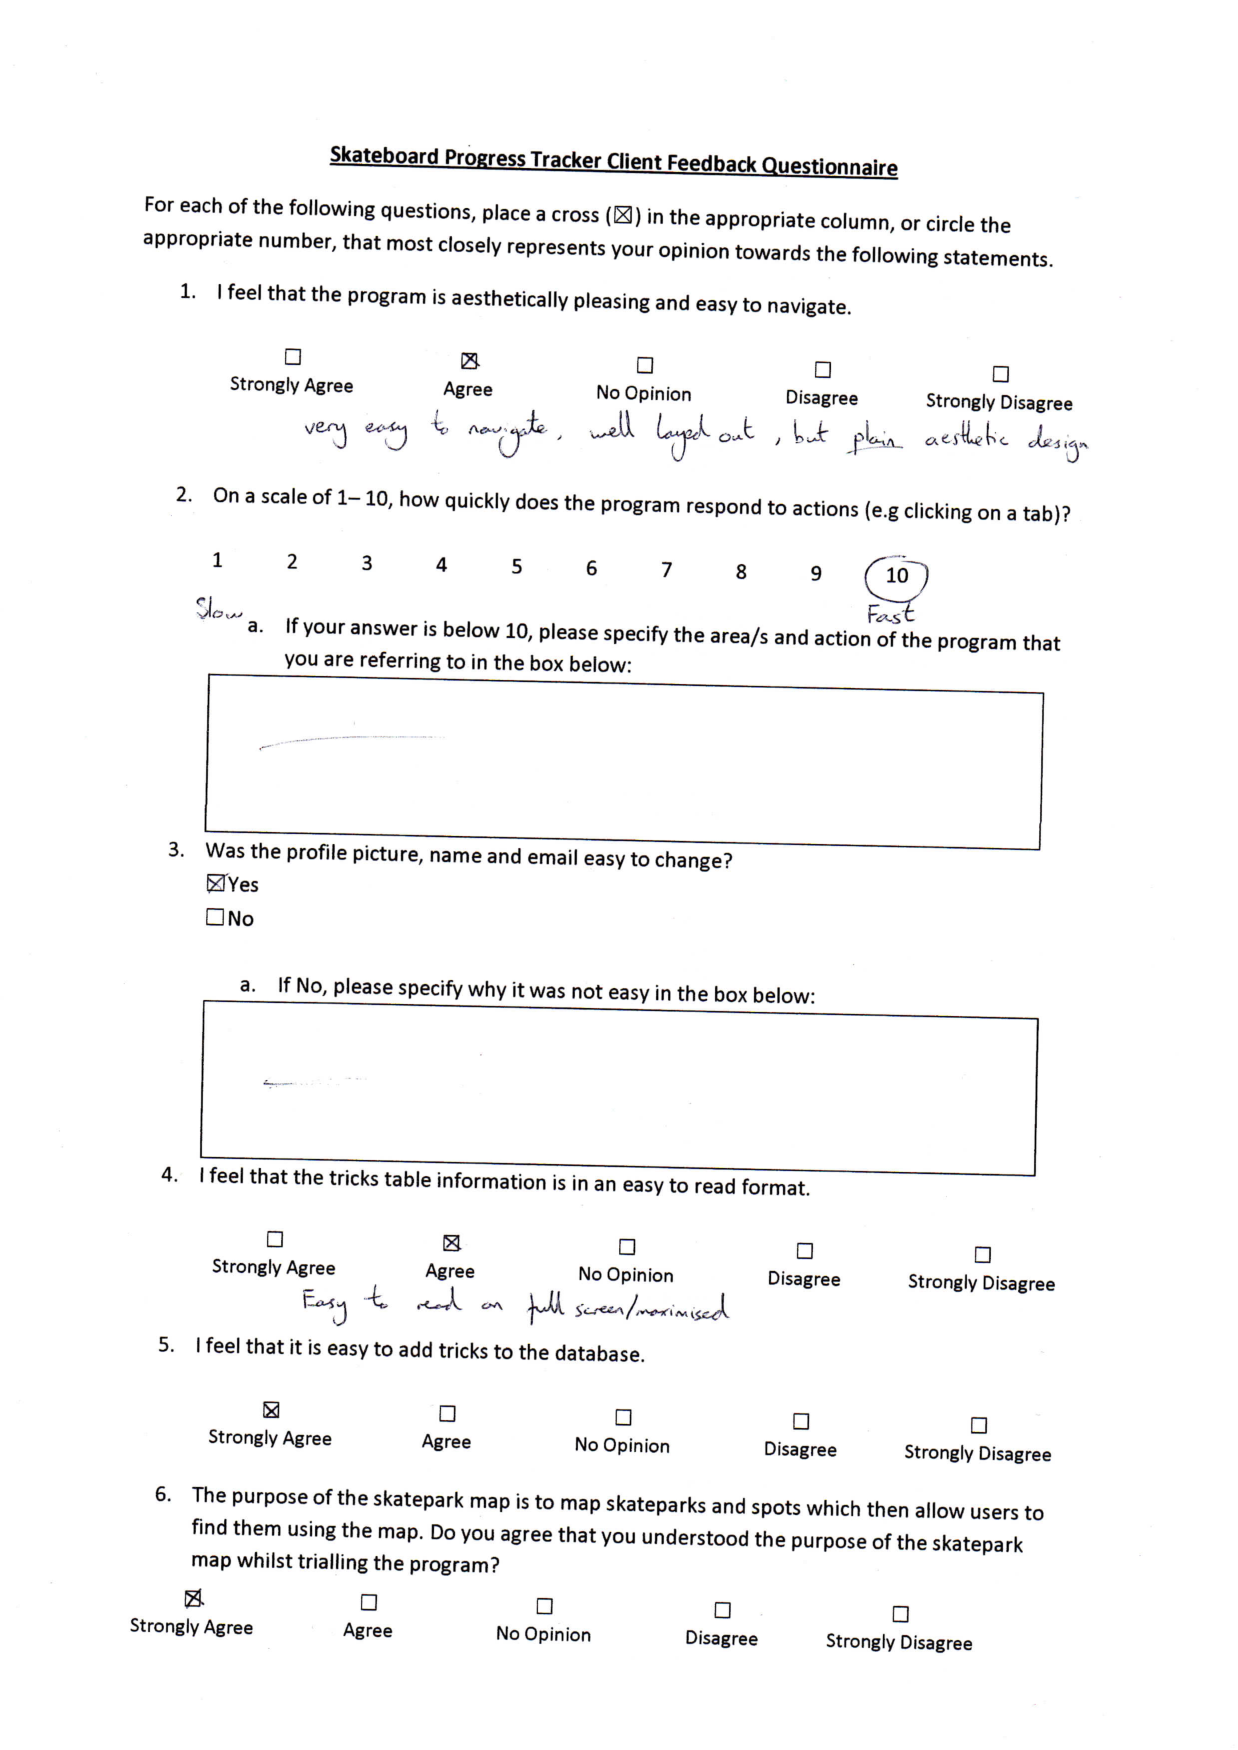
\includegraphics[width=\textwidth]{./Evaluation/images/StuFeedback1.pdf}
    \caption{Stuart Keppie Client Feedback Part 1} \label{fig:StuFeedback1}
\end{figure}

\begin{figure}[H]
    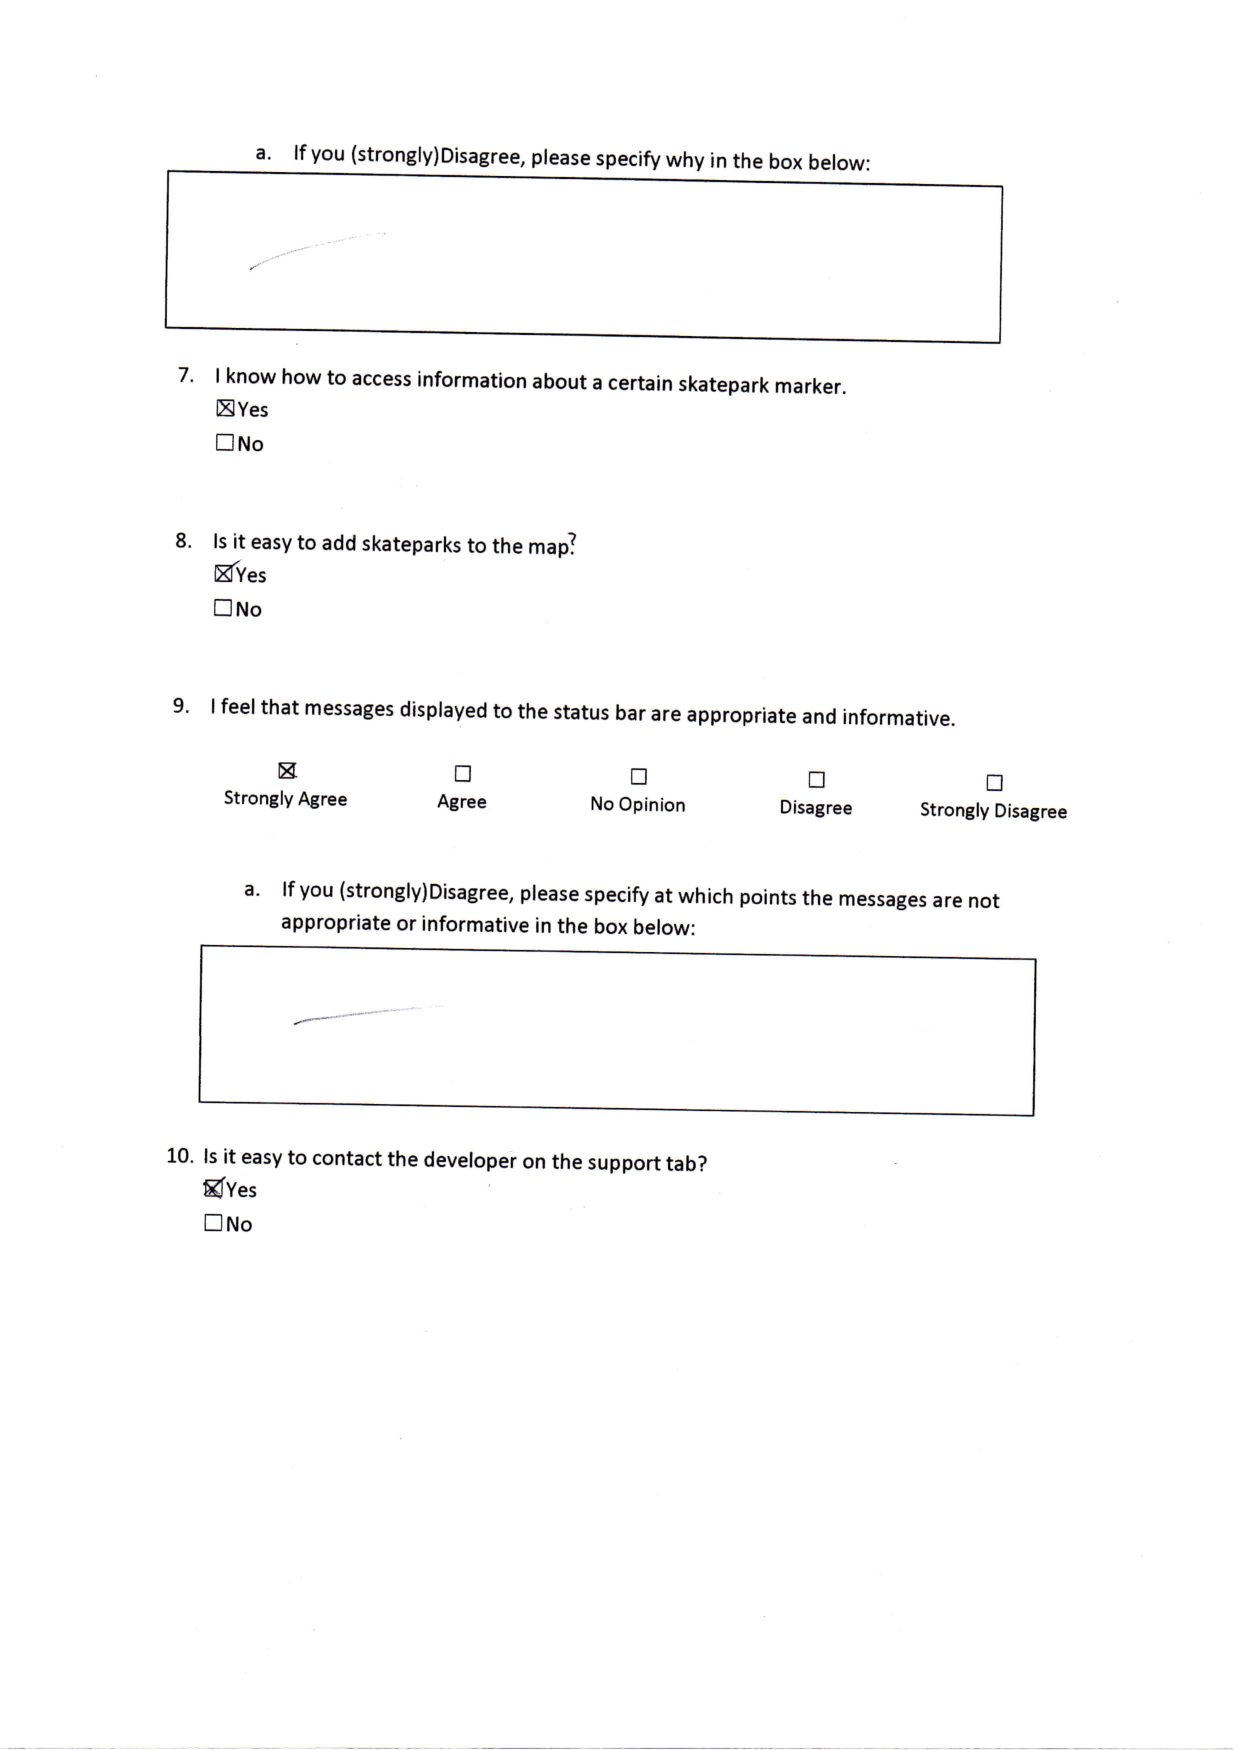
\includegraphics[width=\textwidth]{./Evaluation/images/StuFeedback2.pdf}
    \caption{Stuart Keppie Client Feedback Part 2} \label{fig:StuFeedback2}
\end{figure}

\begin{figure}[H]
    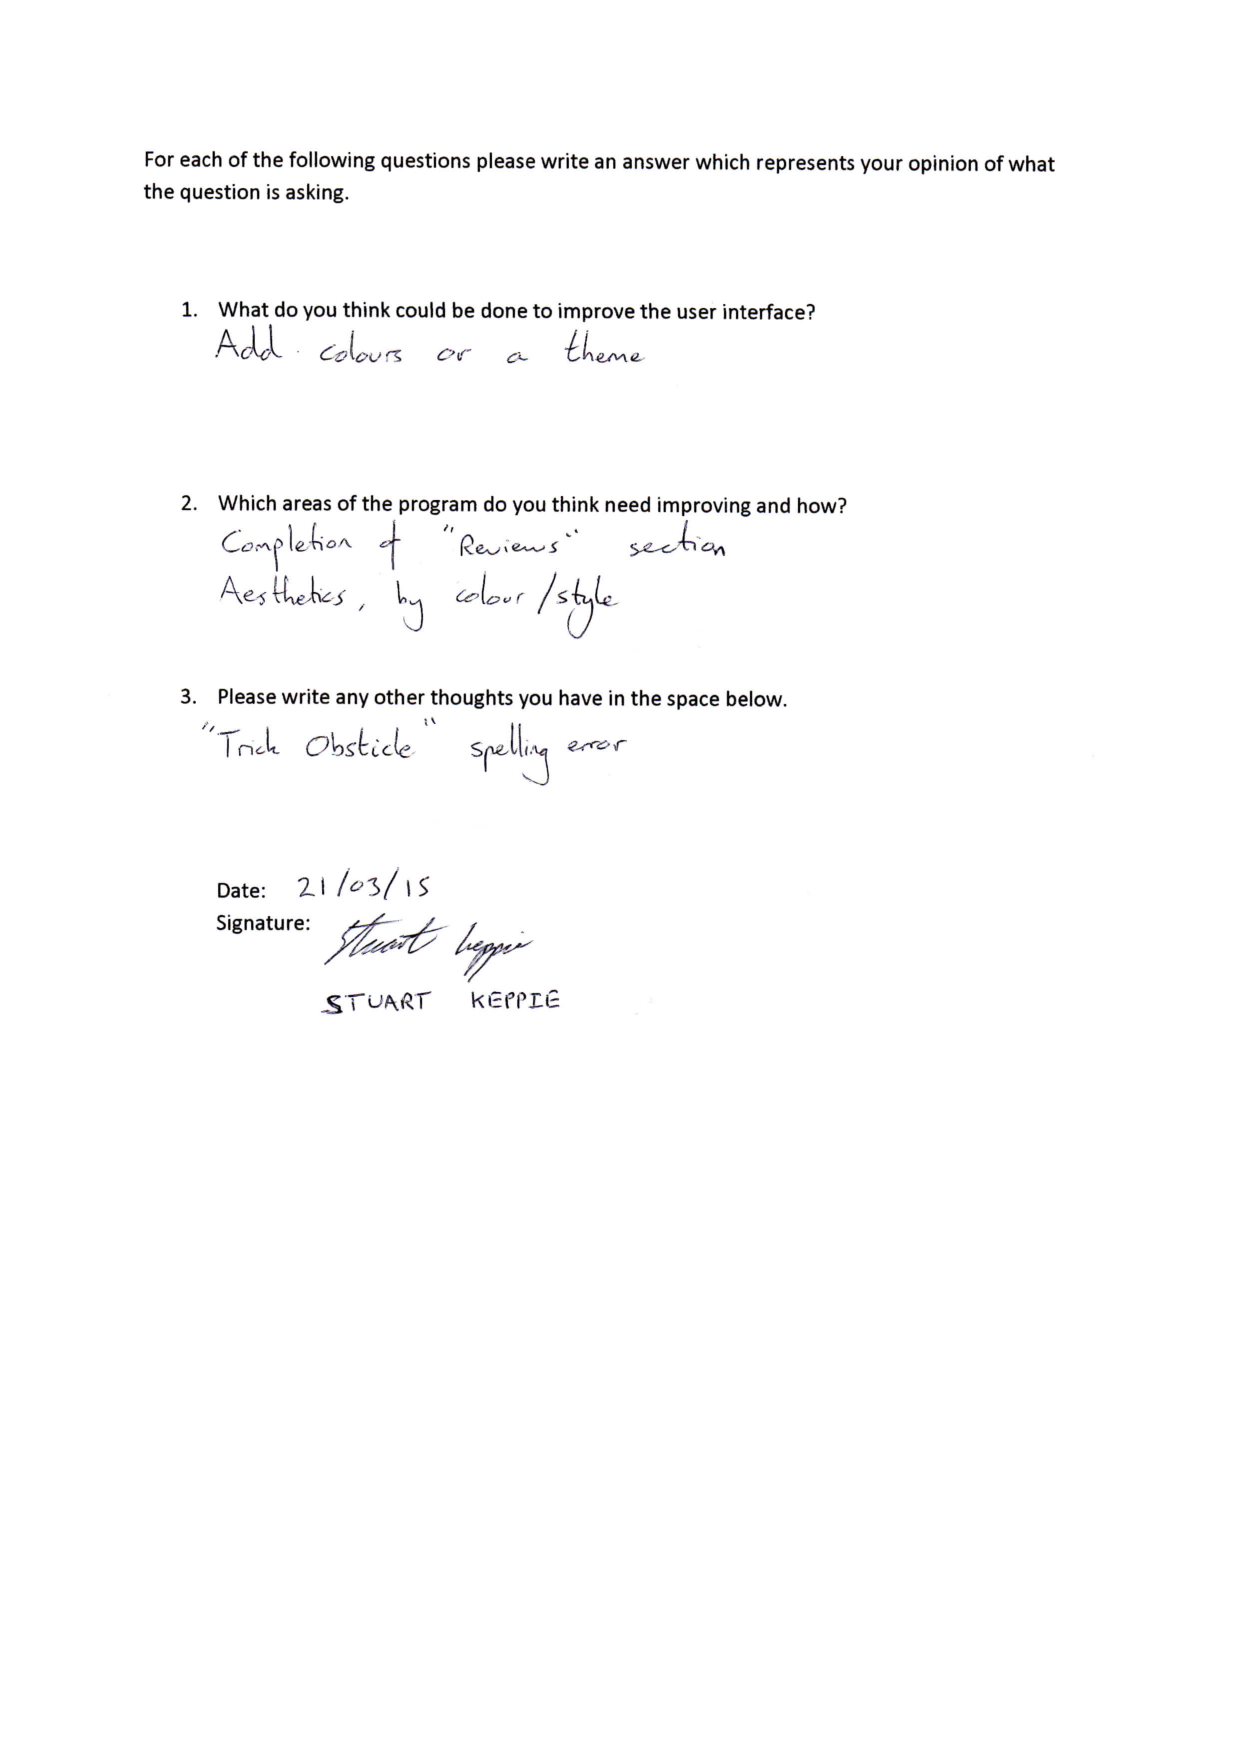
\includegraphics[width=\textwidth]{./Evaluation/images/StuFeedback3.pdf}
    \caption{Stuart Keppie Client Feedback Part 3} \label{fig:StuFeedback3}
\end{figure}

\subsubsection{General Feedback Questionnaire}

\begin{figure}[H]
    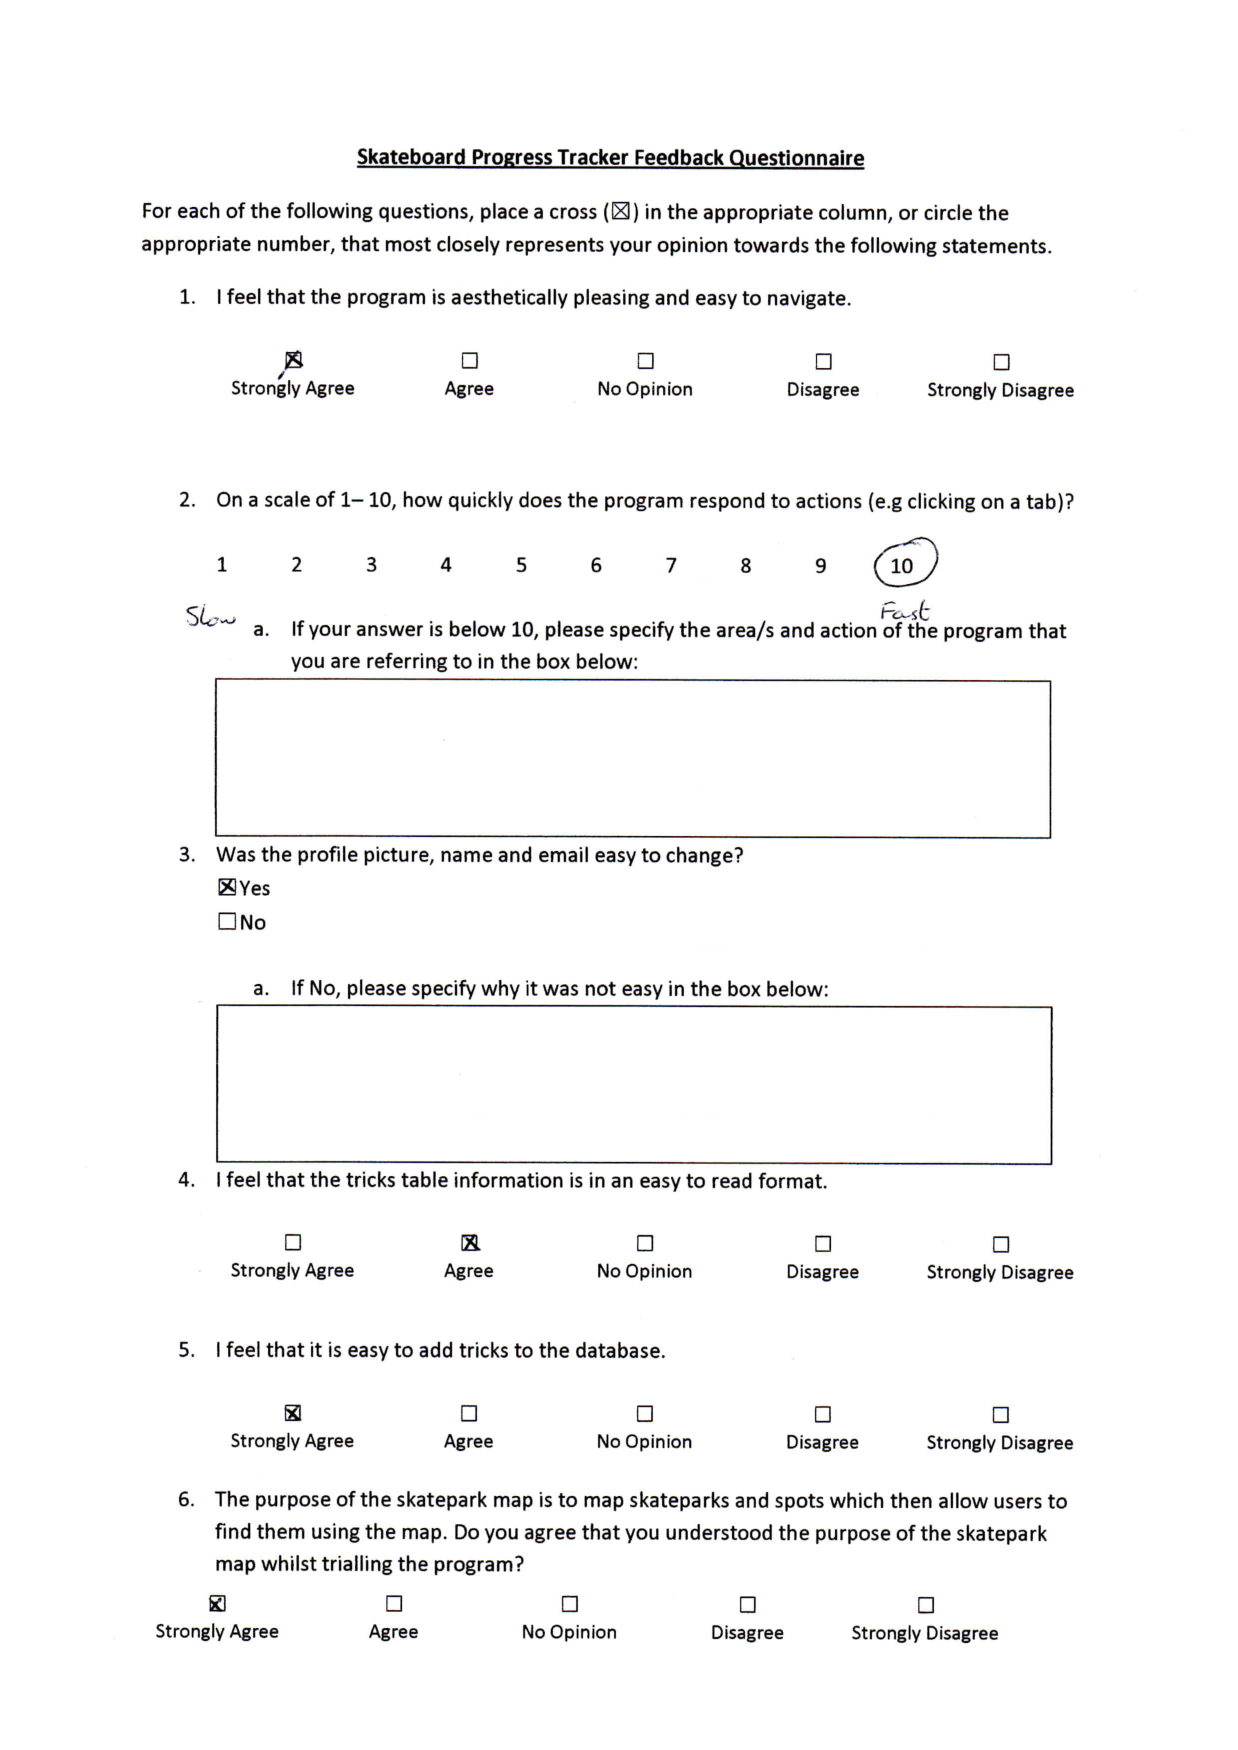
\includegraphics[width=\textwidth]{./Evaluation/images/PierreFeedback1.pdf}
    \caption{Pierre Feedback Part 1} \label{fig:PierreFeedback1}
\end{figure}

\begin{figure}[H]
    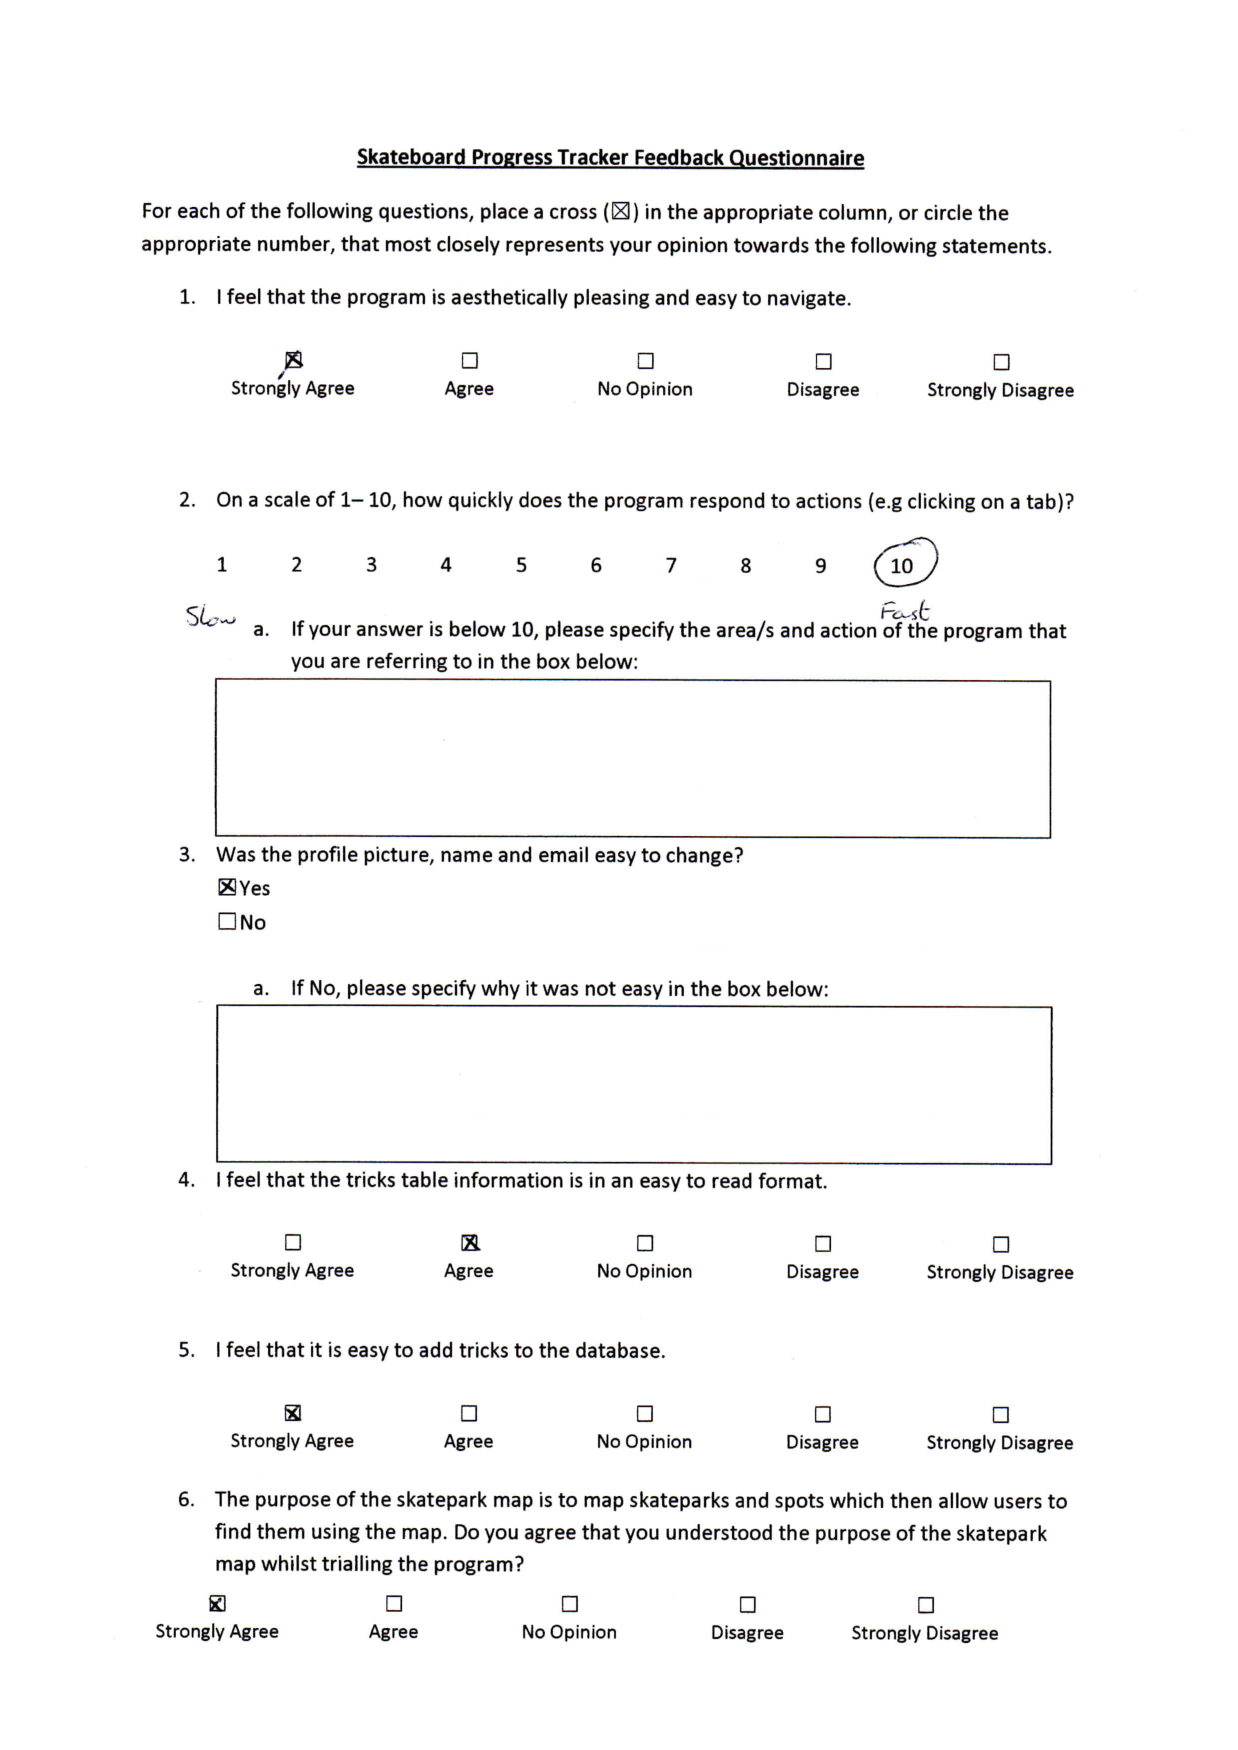
\includegraphics[width=\textwidth]{./Evaluation/images/PierreFeedback1.pdf}
    \caption{Pierre Feedback Part 2} \label{fig:PierreFeedback2}
\end{figure}

\begin{figure}[H]
    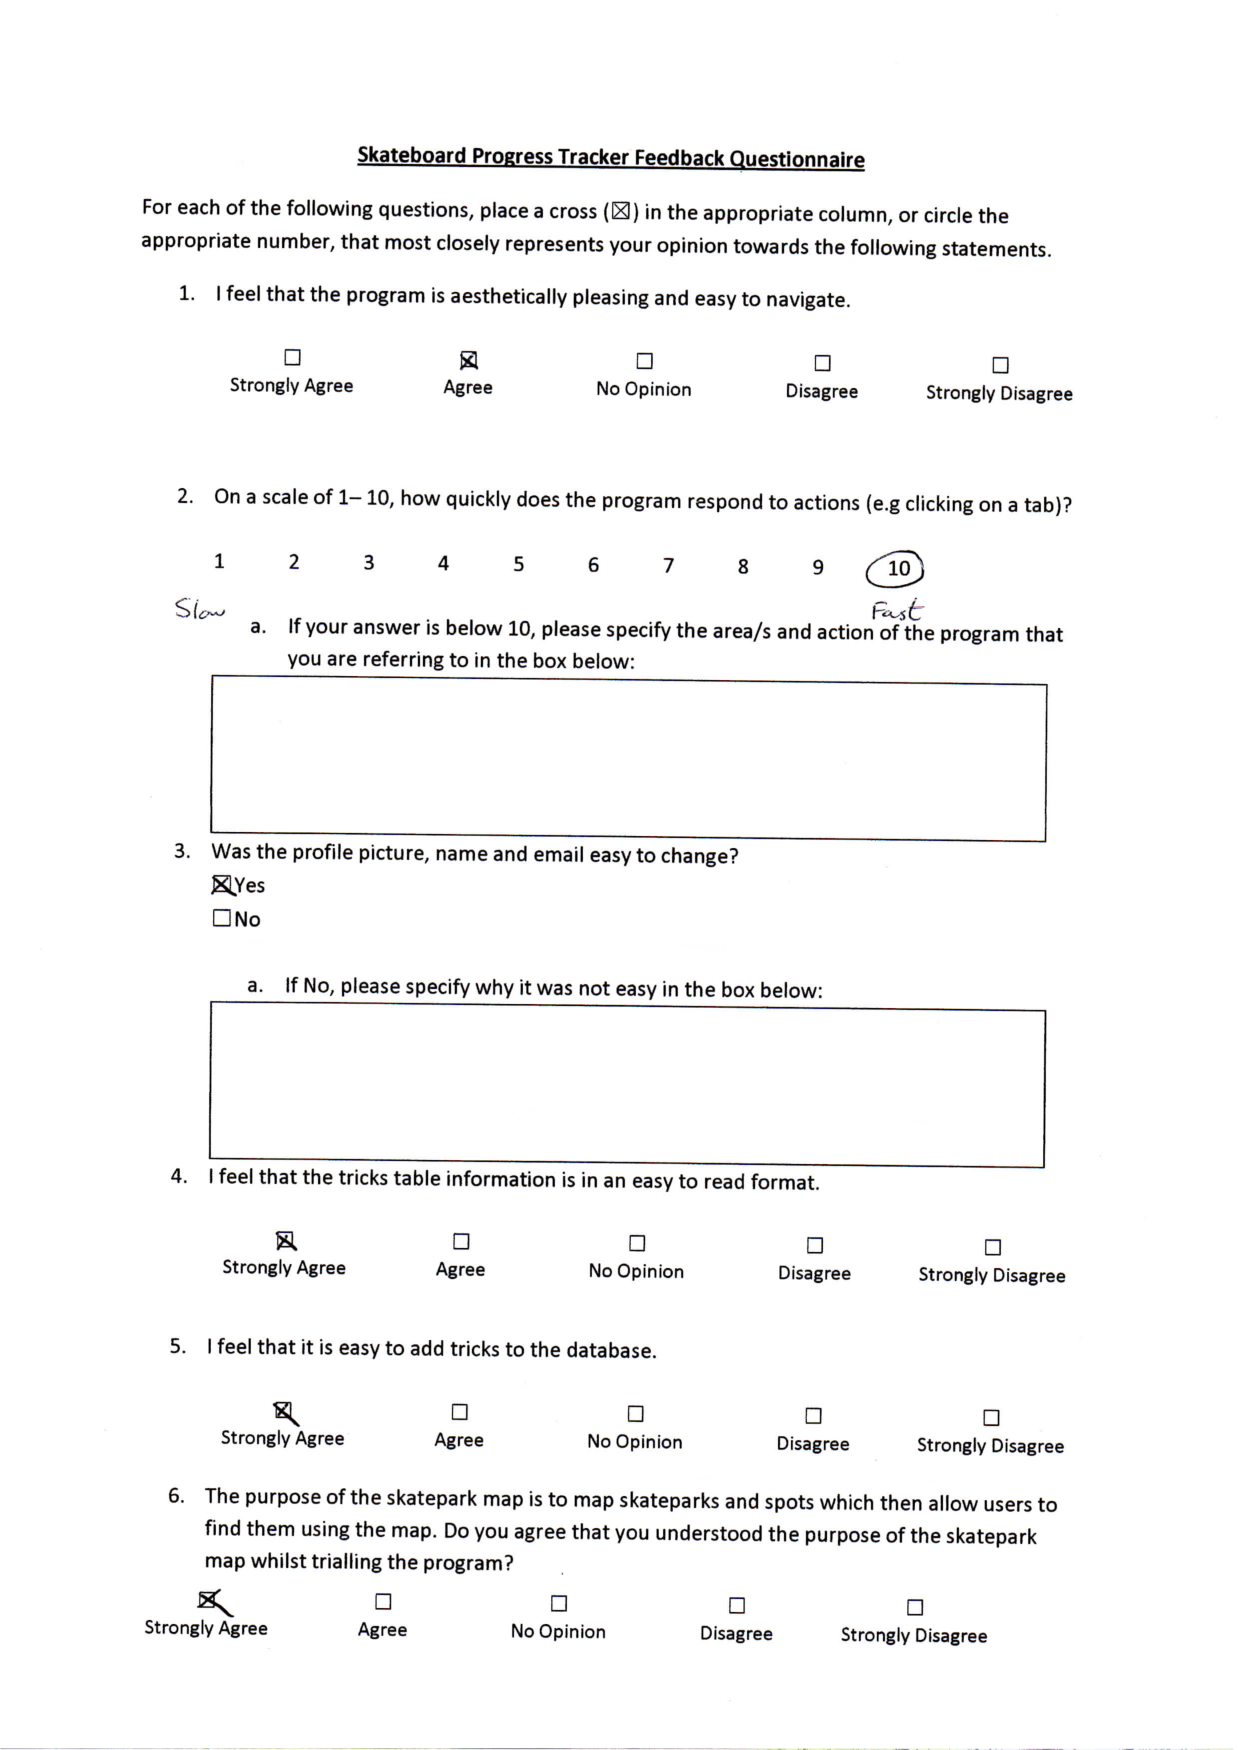
\includegraphics[width=\textwidth]{./Evaluation/images/LeucilleFeedback1.pdf}
    \caption{Leucille Feedback Part 1} \label{fig:LeucilleFeedback1}
\end{figure}

\begin{figure}[H]
    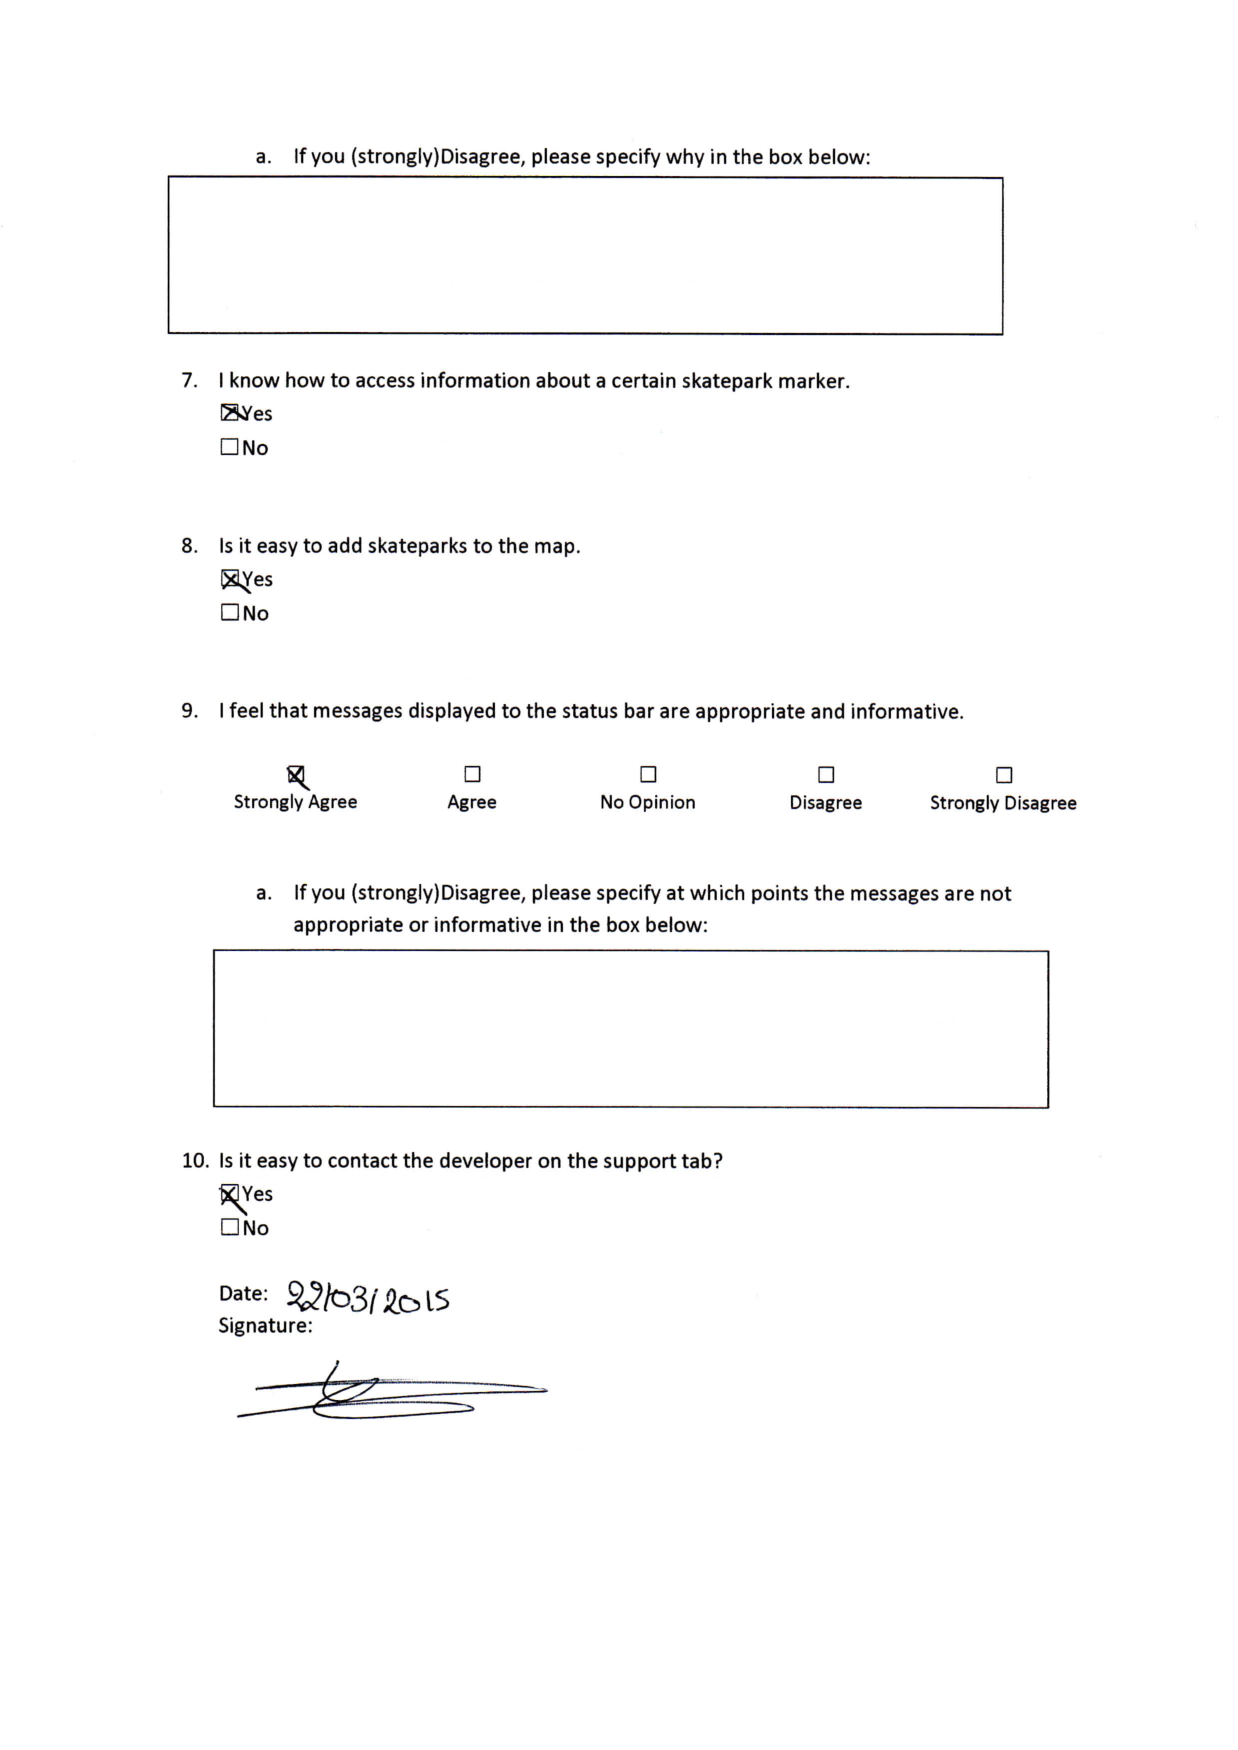
\includegraphics[width=\textwidth]{./Evaluation/images/LeucilleFeedback2.pdf}
    \caption{Leucille Feedback Part 2} \label{fig:LeucilleFeedback2}
\end{figure}

\begin{figure}[H]
    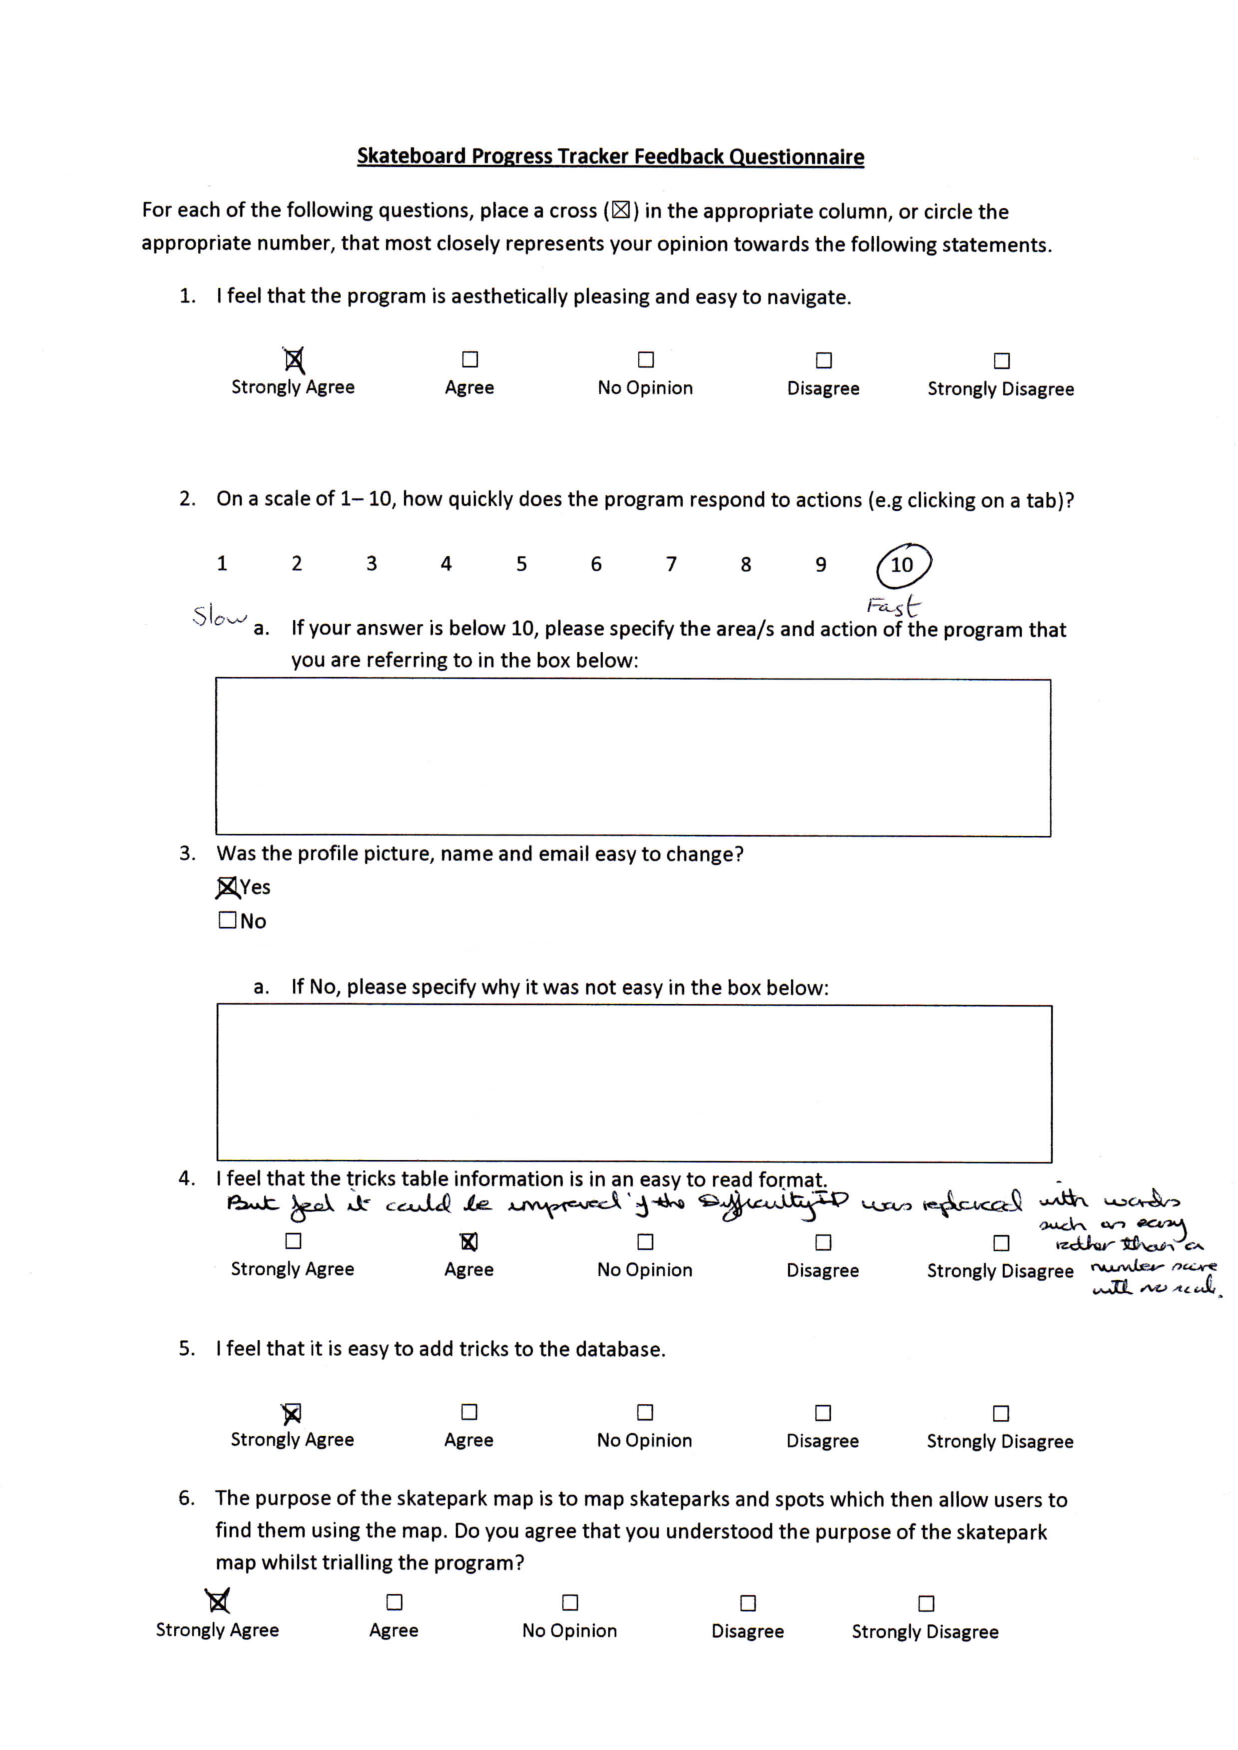
\includegraphics[width=\textwidth]{./Evaluation/images/SueFeedback1.pdf}
    \caption{Sue Feedback Part 1} \label{fig:SueFeedback1}
\end{figure}

\begin{figure}[H]
    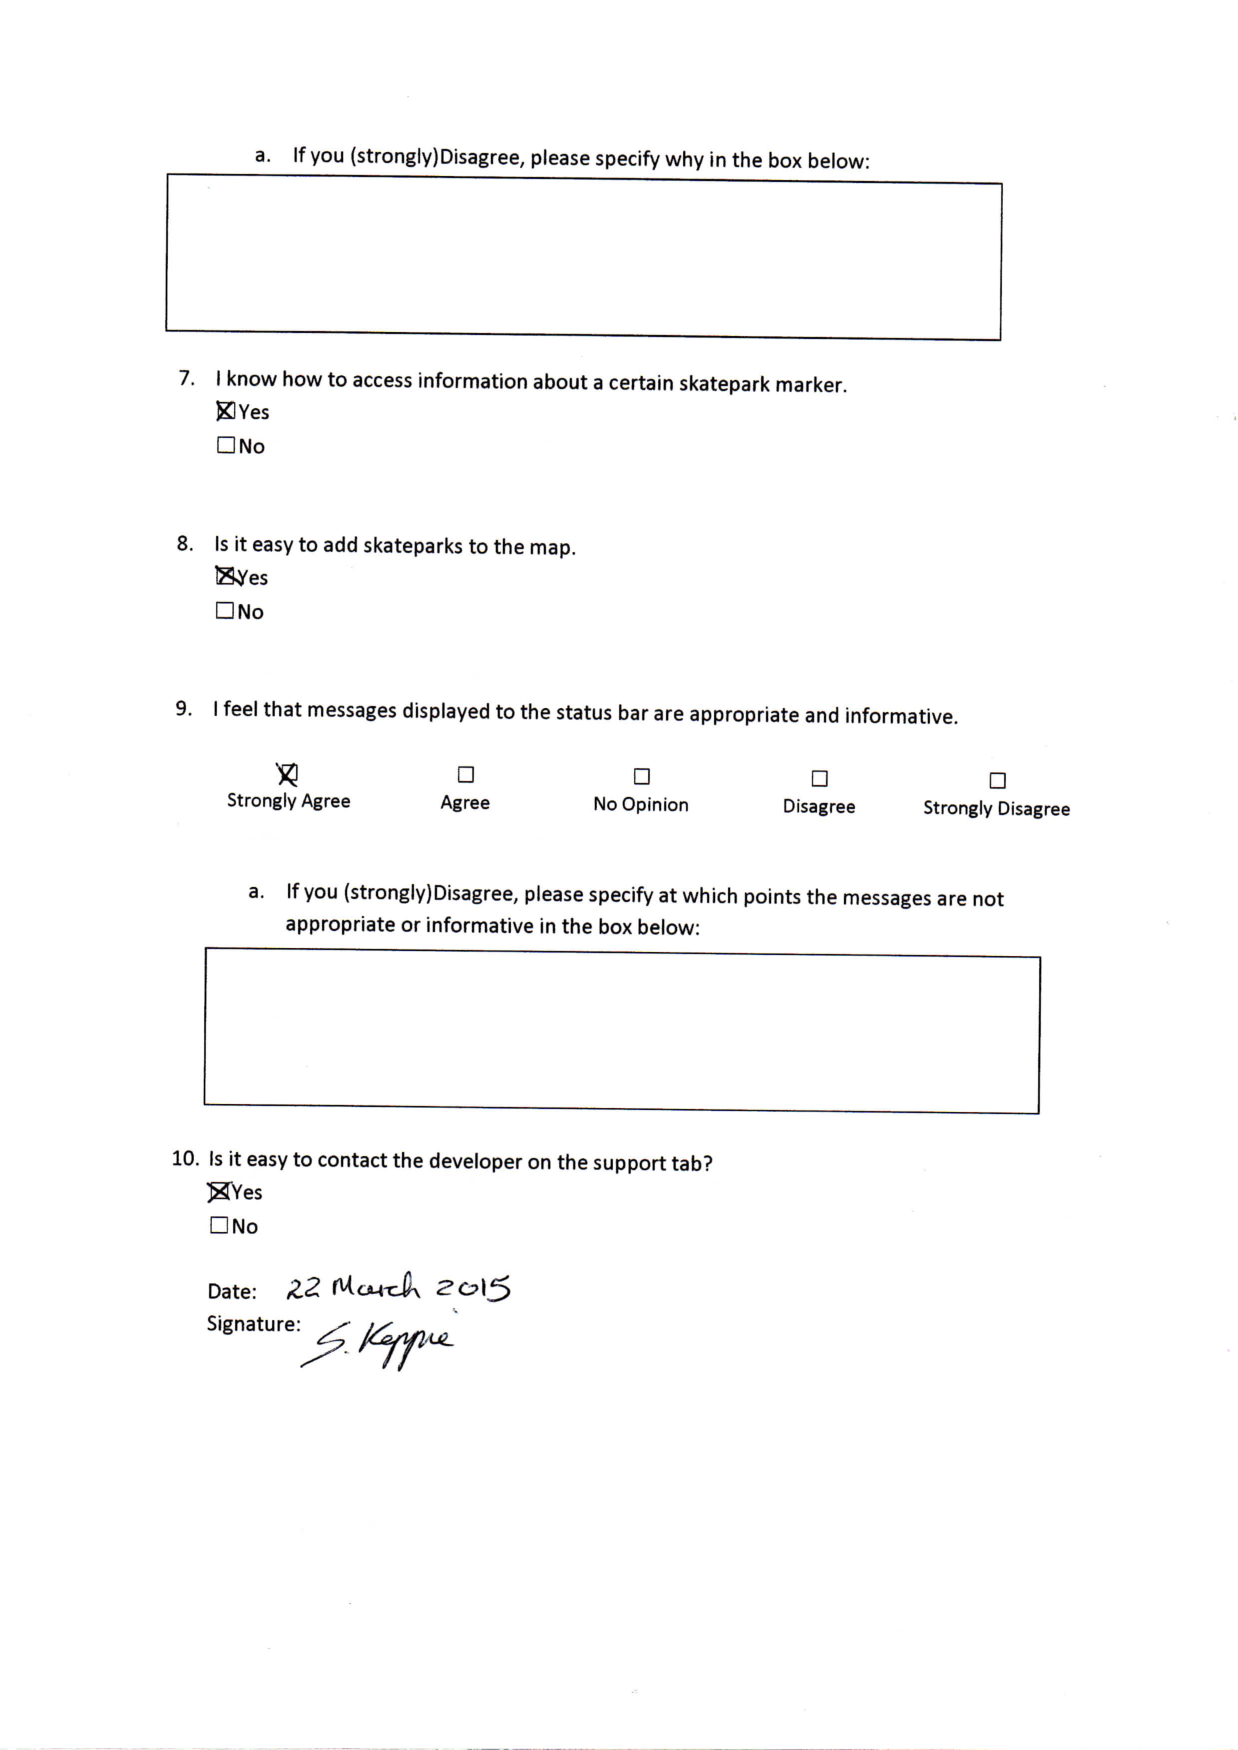
\includegraphics[width=\textwidth]{./Evaluation/images/SueFeedback2.pdf}
    \caption{Sue Feedback Part 2} \label{fig:SueFeedback2}
\end{figure}



\subsection{Graphs}

\begin{figure}[H]
    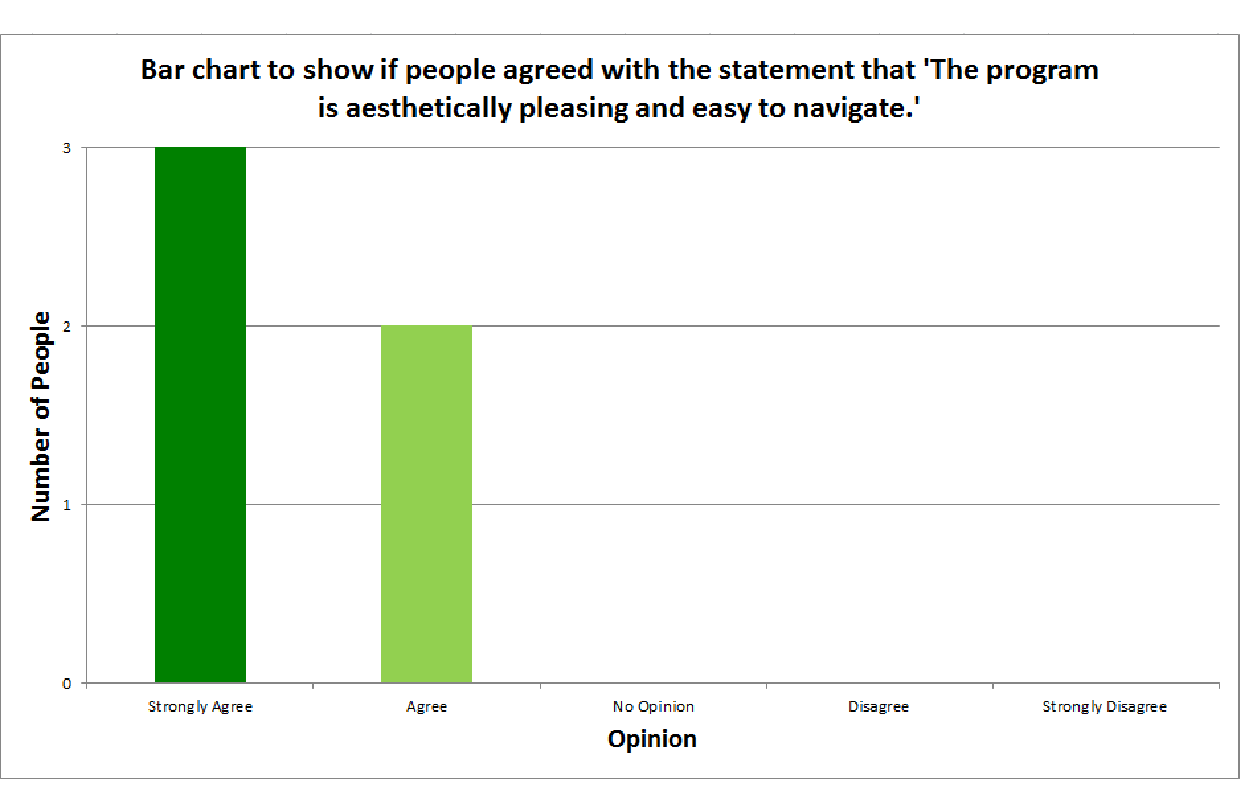
\includegraphics[width=\textwidth]{./Evaluation/images/AestheticsGraph.pdf}
    \caption{Bar Chart for Aesthetics and Navigation Opinions.} \label{fig:AestheticsGraph}
\end{figure}

\begin{figure}[H]
    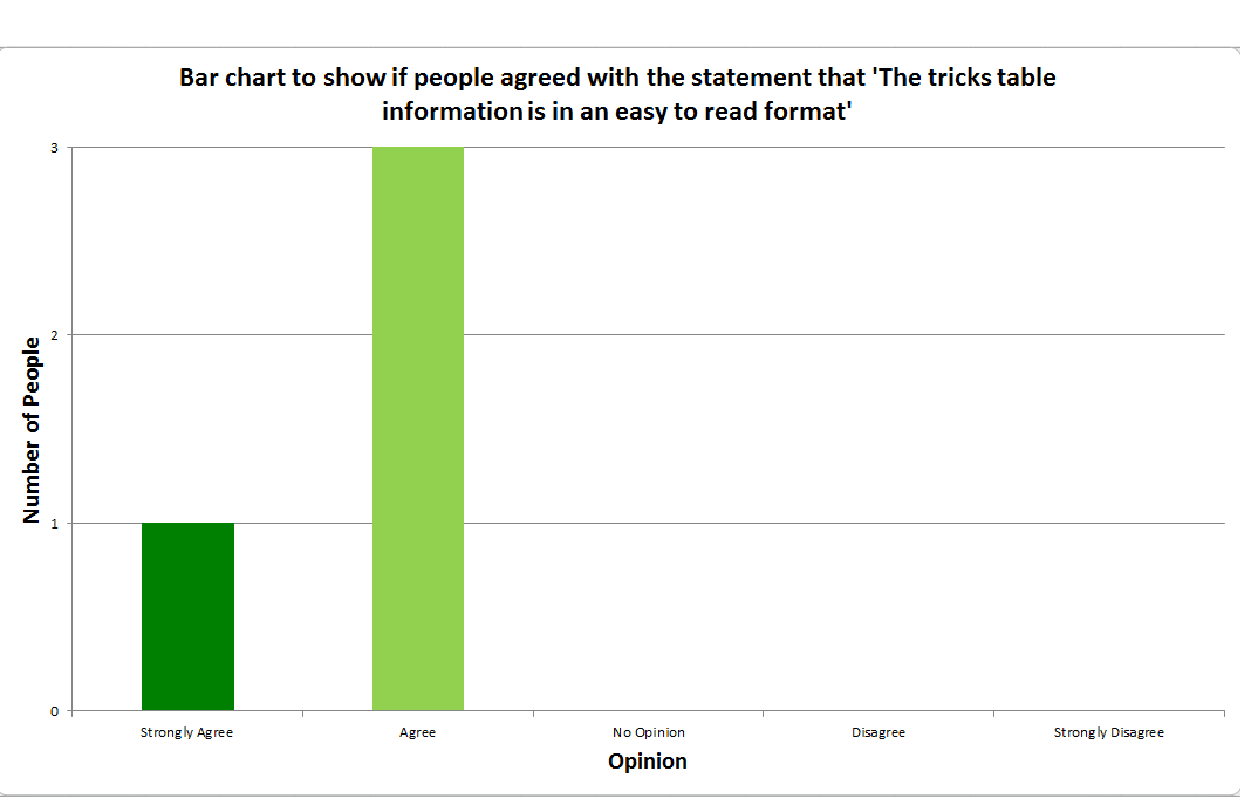
\includegraphics[width=\textwidth]{./Evaluation/images/TricksTableGraph.pdf}
    \caption{Bar Chart for Tricks Table Format} \label{fig:TricksTableGraph}
\end{figure}


\subsection{Written Statements}

The written statements that I received are included within my questionnaire in section \ref{QSub} on page \pageref{QSub}.
